\section{Parallel Partitioning and Sampling}\label{sec:parallel_partitioning_and_sampling_of_the}

% dedicated solver

The derivation of increasingly detailed models in the domain of biomechanics has to be complemented by engineering of efficient software that is used to solve these models. Using proper parallelization allows to increase the amount of computational load that is possible to handle. In turn, this allows to simulate more complex models with higher resolution and ultimately enables physiological and pathological insights on a new level.

For detailed multi-scale model solvers, parallelization is a complex task. 
The paradigm has to be regarded  during the whole setup process of the system. Different descriptions for the same physical behavior have to be evaluated with respect to their solvability in parallel. For a given model, suitably parallelizable numerical solution schemes have to be selected. The implementation of individual solvers and their coupling have to take into account the parallel environment. 
Discretization schemes enabling parallel domain decomposition are required. Their representation on compute hardware with distributed memory has to be taken into account as well as ensuring acceptable conditioning of large scale problems. To ensure fast runtimes, load balancing between compute nodes and parallel scalability are important.

All these fundamental considerations potentially depend on each other and require a comprehensive solution. 
Thus, it is often difficult to port existing, isolated solver software that was designed for serial or moderately parallel execution to efficiently fit into a highly-parallel, multi-scale solution framework. To not (re-)create this kind of isolated solvers for individual model components, we focus on their parallel design from the ground up in the current and following sections.

In this section, we introduce algorithms for the generation of parallel partitioned meshes, which are fundamental ingredients to all our solvers. \Cref{sec:algorithm_for_partitioning_and_sampling,sec:partitioning_requirements} set the scene and define our requirements for well-behaved parallelized meshes. \Cref{sec:partitioning_alg1,sec:partitioning_alg2} give details on the implemented algorithms and \cref{sec:partitioning_user_options} addresses the configuration for the user. \Cref{sec:partitioning_results} concludes by comparing the resulting partitionings for different parameters.

Afterwards, \cref{sec:parallel_partitioning_for_fiber_based,sec:parallel_solver_multidomain} TODO present dedicated parallel solvers for various parts of the multi-scale model. Sections (TODO: reference) describe structures that are needed for the interplay of the individual model components.


%\subsection{Algorithm for Partitioning and Sampling the 3D Mesh}\label{sec:algorithm_for_partitioning_and_sampling}
\subsection{Specification of the Partitioning}\label{sec:algorithm_for_partitioning_and_sampling}

Structured meshes of the types \code{RegularFixed}\code{OfDimension<D>} or \code{Structured}\code{Deformable}\code{OfDimension<D>} are partitioned for parallel execution by distributing the elements to all processes. As mentioned in \cref{sec:oragnization_of_parallel_partitioned_data}, planar cuts in the space of the element indices separate the subdomains. For example, in computations on a structured 3D mesh with $N_x^\text{el} \times N_y^\text{el} \times N_z^\text{el}$ global elements, the process with rank $r$ owns a subdomain with
$N_x^{\text{el,local,}r} \times N_y^{\text{el,local,}r} \times N_z^{\text{el,local,}r}$ local elements.
The sizes of the local subdomains depend on the specified total number of subdomains $n_i$ in each coordinate direction $i \in \{x,y,z\}$.
Given $n_i$, the number of local elements in every subdomain along the coordinate axis $i$ can be set to either $N_i^{\text{el,local}} = \lfloor N^\text{el}_i/n_i+1\rfloor$ or $N_i^{\text{el,local}} = \lfloor N^\text{el}_i/n_i \rfloor$ to allow for good load balancing.

A prerequisite to construct such a partitioning for $n_\text{proc}$ processes is to fix the numbers of subdomains $n_x \times n_y \times n_z = n_\text{proc}$. In OpenDiHu, the Python settings file can either specify the global numbers $N_i^\text{el}$ of elements or separate local numbers $N_i^{\text{el,local,}r}$ of elements for every rank $r$. This step involves setting the option \code{inputMeshIsGlobal} to either \code{True} or \code{False} as explained in \cref{sec:exemplary_usage_1}.

Specifying the global numbers of elements is often useful for toy problems when the total element count is small and the actual partitioning is not important. In this case, PETSc is used to determine optimal subdomain sizes for all processes and, subsequently, constructing the partitioning. Because the partitioning is not yet known at the time of parsing of the Python settings, spatial information such as node positions or boundary conditions have to be specified on every rank for the whole domain.

Most of the electrophysiology examples, however, use the specification of local numbers of elements. Thus, every rank only needs to specify the local data of its subdomain, such as node positions and boundary conditions. This is a prerequisite for good parallel weak scaling behavior as the amount of data processing on each process stays constant when simultaneously increasing problem size and total process counts.

In the electrophysiology examples, the partitioning into $n_x \times n_y \times n_z$ subdomains can be specified by the command line parameter \code{--n_subdomains n_x n_y n_z}, where \code{n_x}, \code{n_y} and \code{n_z} are replaced by the actual numbers. Their product has to match the process count $n_\text{proc}$ that is given to MPI to start the program.
If this option is not specified, the values are determined automatically by the following algorithm: For all partitions of the number $n_\text{proc}$ into three integer factors, a performance value $p$ is computed as follows:
%
\begin{align*}
  p = (n_x-n_\text{opt})^2 + (n_y-n_\text{opt})^2 + (n_z-n_\text{opt})^2.
\end{align*}
The optimal value is given by $n_\text{opt} = n_\text{proc}^{1/3}$. The partitioning with the lowest value of $p$ is selected among all partitions as it leads to subdomains with the best volume-to-surface ratio for a cube-shaped domain. An advantage of this method is that it is independent of the mesh size.

\subsection{Requirements for Partitioning and Sampling of the 3D Mesh}\label{sec:partitioning_requirements}

Simulation scenarios with fiber-based electrophysiology use a 3D muscle mesh and embedded 1D fiber meshes that are generated from the same node positions, as described in \cref{sec:postprocessing_of_the_generated_streamlines}. The binary input file contains a structured grid of points that can be either interpreted as 1D fibers by connecting the points in $z$-direction or as 3D mesh by additionally connection points in $x$ and $y$-directions.

Usually, all points in such a file are used to define the 1D fiber meshes and the 3D mesh is constructed from only a subset of the available points. To obtain a 3D mesh with approximately equal mesh widths in all coordinate directions, the point data is sampled by constant strides in $x$, $y$ and $z$ direction.  The stride in fiber direction ($z$ direction) is typically chosen larger than the strides in transverse directions as the distance between the given points is smaller in this direction.

In the following, we discuss the sampling procedure that generates the partitioned 3D mesh from the fiber data in more detail.
Given a structured hexahedral fine 3D mesh, numbers of subdomains $n_i$ and sampling stride parameters \code{sampling_stride_$i$} for the three coordinate directions $i\in\{x,y,z\}$, we have to determine the nodes that should be part of each subdomain in the resulting coarser hexahedral 3D mesh. 

For illustration, \cref{fig:partitioning1} shows the initial fine mesh consisting of spheres that are arranged in fibers that run from the shown cross section to the back. The resulting sampled mesh is given by the white elements and uses a subset of the nodes in the fine mesh. The sampled mesh is parallel partitioned into the colored subdomains. 
Furthermore, the coarse mesh consists of quadratic elements that are formed from two by two white elements in the cross section each. Hence, every subdomain contains an even number of the white elements in horizontal and vertical directions.

% quadratic partitioning
\begin{figure}
  \centering%
  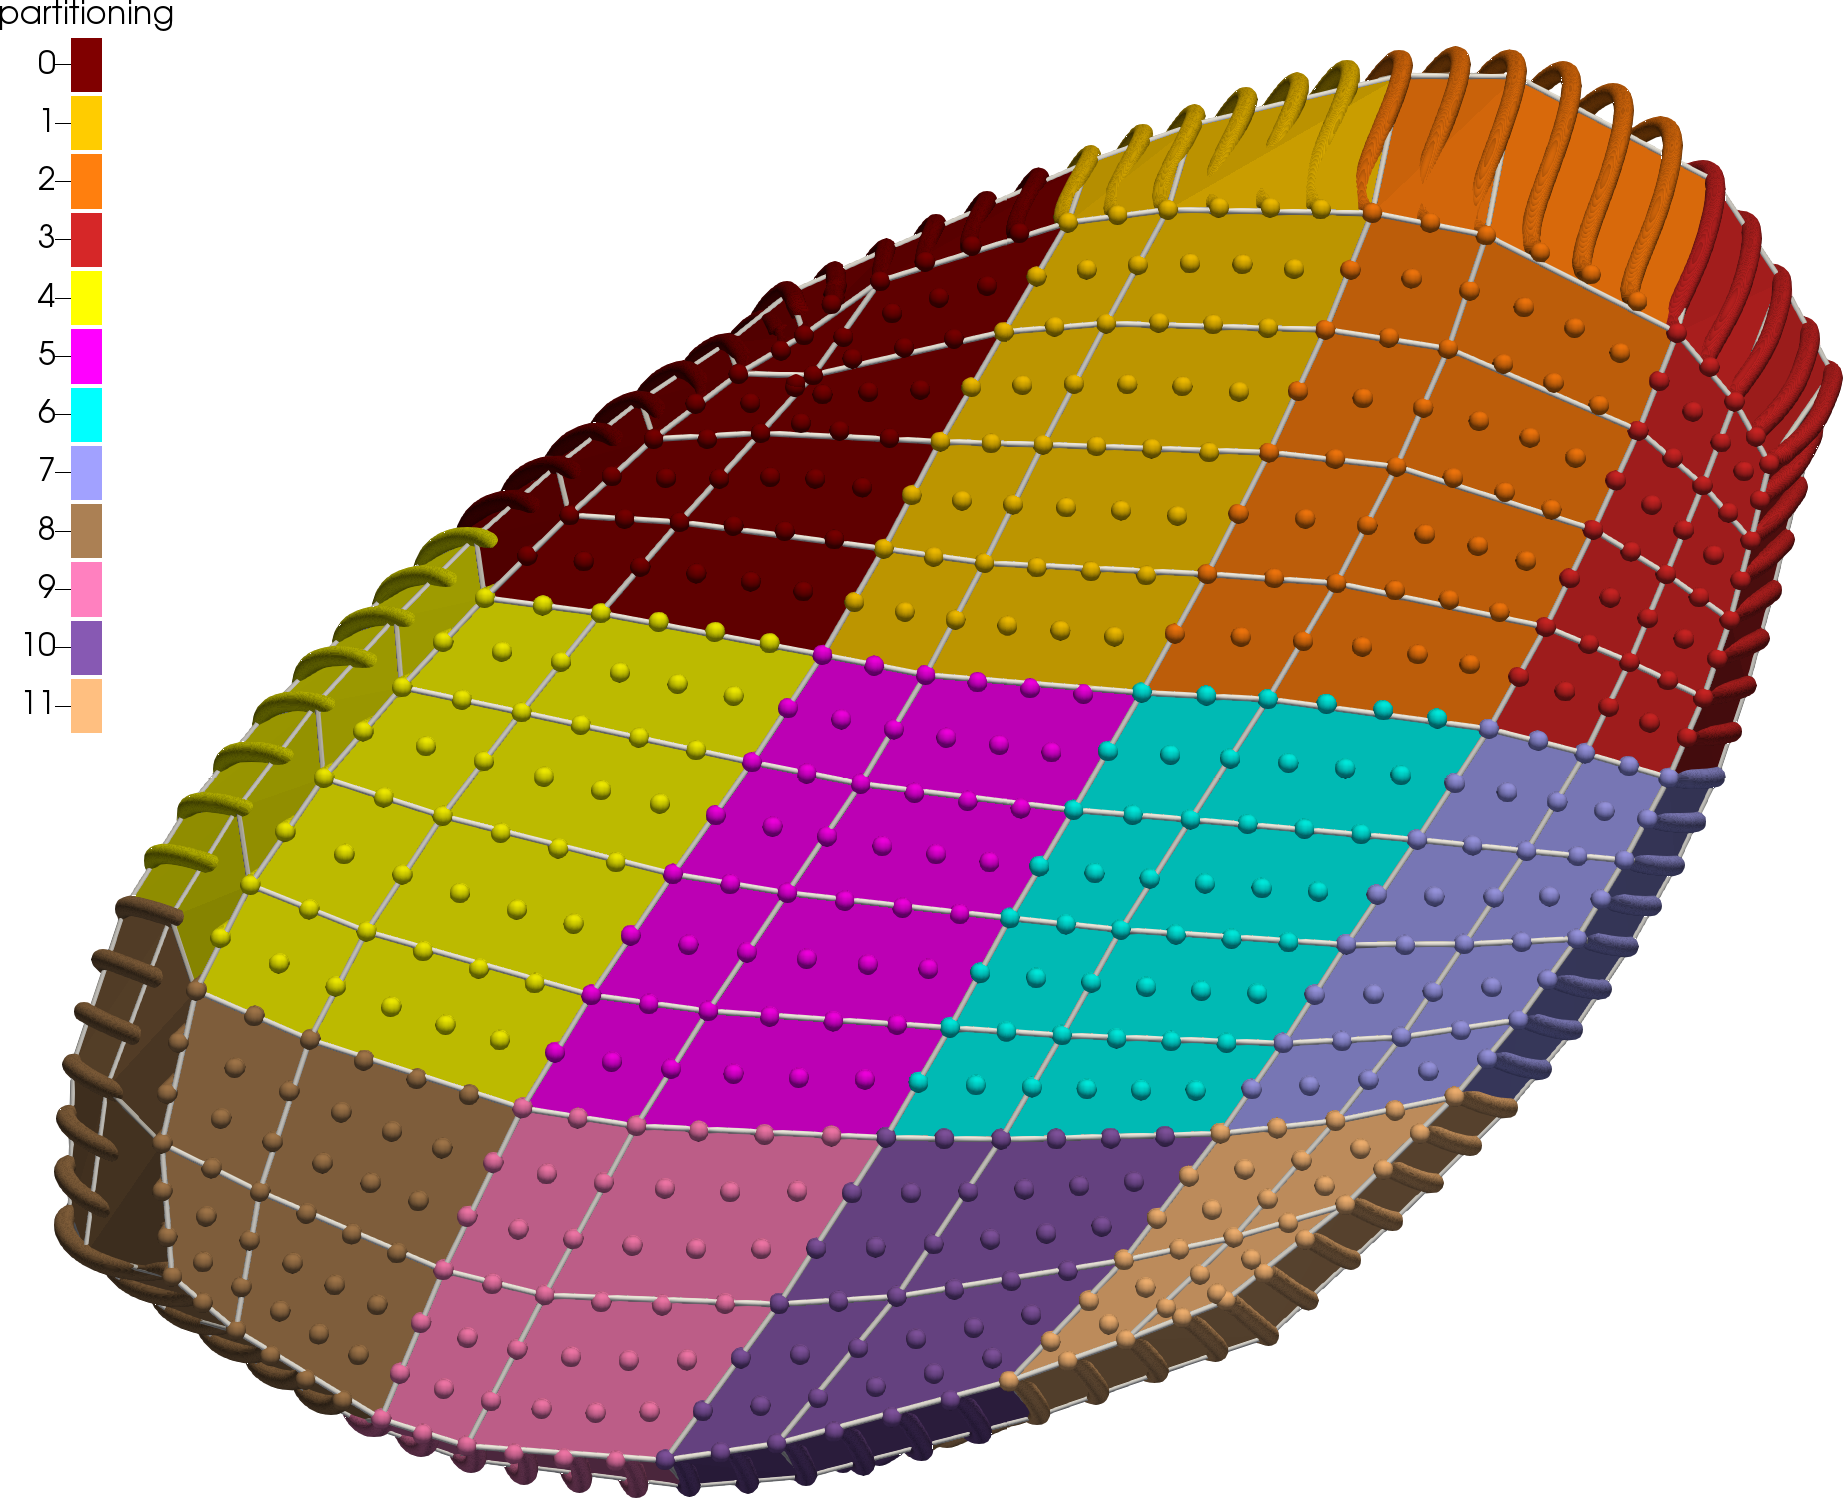
\includegraphics[width=\textwidth]{images/implementation/partitioning7.png}%
  \caption{Partitioning and subsampling of a fiber mesh to twelve proceses. The fiber data indicated by the spheres is sampled with a stride parameter of two to obtain the partitioned quadratic coarse mesh given by the white elements. The subdomains are indicated by different colors.}%
  \label{fig:partitioning1}%
\end{figure}%

The requirements to the sampling and partitioning algorithm are as follows: 
\begin{enumerate}[label=(\roman*)]
\item The resulting coarser 3D mesh should use every $k$th node where $k$ is adjustable by the parameter \code{sampling_stride_$i$} in the settings.
\item The number of nodes in every subdomain should be approximately equal to allow for a good load balancing in the computation.
\item There should be as little \say{remainder elements} that have a different mesh width than the majority of the elements as possible.
\item If a quadratic mesh is required, e.g., for solid mechanics models, the number of (linear) elements in every subdomain in every coordinate direction has to be even to allow for the generation of quadratic hexahedral elements.
\end{enumerate}

Clearly, not all requirements can be fulfilled exactly for all given input meshes. For combinations of given input mesh sizes and sampling strides that lead to an even number of sampled nodes, requirement (iv) cannot be fulfilled. 
Exact fulfillment of requirement (ii), i.e., an equal number of nodes in every subdomain is also only possible for suited parameter choices. Therefore, we relax requirement (i) and also occasionally allow different step widths between the selected nodes on the fine grid. Having varying distances between the nodes leads to elements with different mesh widths, which is unfavorable in terms of the numeric conditioning of the problem. Therefore, the number of such elements should be as low as possible, which is also stated by requirement (iii).

To avoid differently sized elements as possible, we work with a granularity parameter. This parameter specifies the amount of nodes to summarize and treat as an indivisible unit. For example, a value of \code{granularity_x=2} specifies that always two neighboring points are in the same element. Then, subdomain boundaries and element boundaries can only occur at every second node.

\subsection{Algorithm for Determining the Subdomains}\label{sec:partitioning_alg1}

Important steps in the algorithm for sampling the fine mesh and constructing the partitioning are, first, to determine the locations of the new subdomains in the original fine grid, second, to determine the number of sampled points in each subdomain and third, to determine which points from the fine grid will be sampled in every subdomain of the coarse grid. The steps have to be carried out independently for all three coordinate directions. Thus, it suffices to only consider the algorithm for the partitioning along one axis.
In the following, we present the algorithms of the first two steps for the $x$-axis. 

The algorithm for the first step is given in \cref{alg:n_fibers_in_subdomain}. Input to the function \code{n_fibers_in_}\code{subdomain_x} is a subdomain coordinate in the range $[0,n_x-1]$ that identifies the subdomain. The output to be computed is the number of grid points in the fine grid or equivalently, the number of fibers that are contained in the subdomain. Calling this function for all subdomains defines the partitioning of the fine grid.

% partitioning algorithm
\begin{figure}
  \centering%
  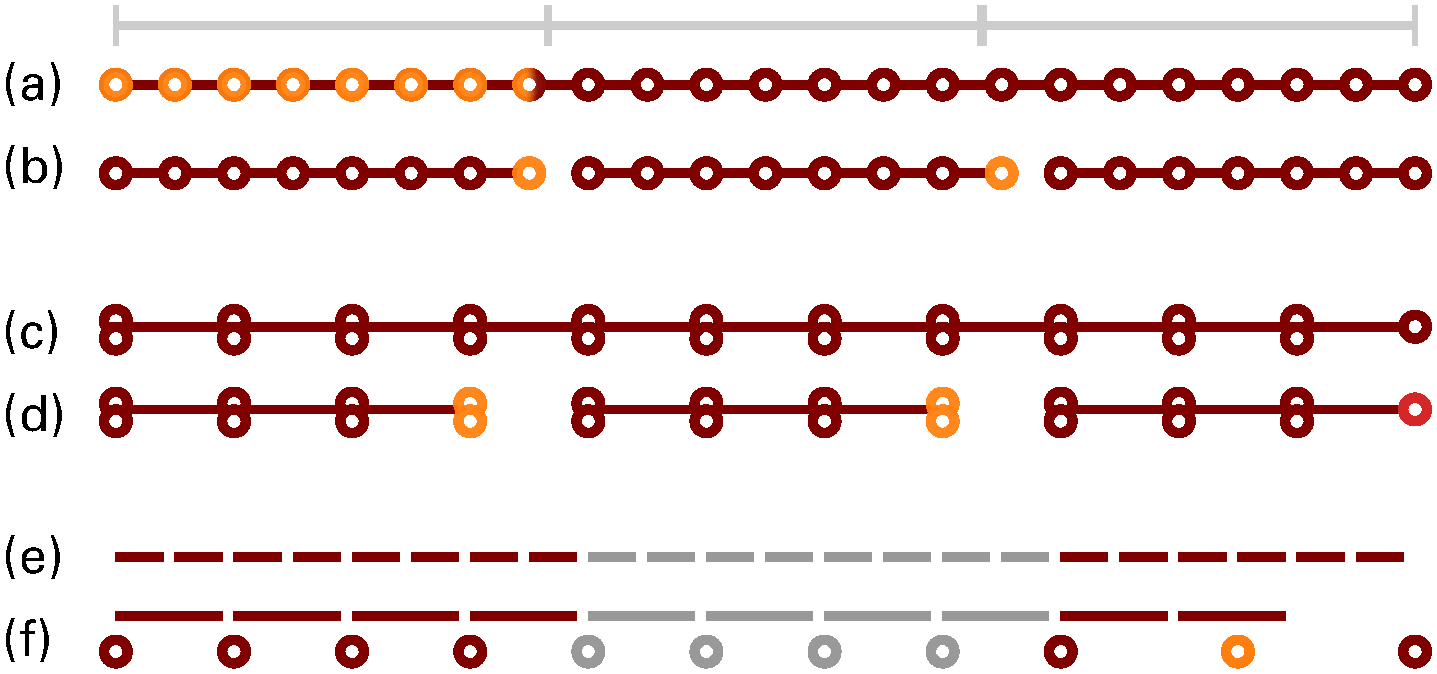
\includegraphics[width=\textwidth]{images/implementation/partitioning_algorithm.pdf}%
  \caption{Visualization of the steps of the partitioning algorithms given by \cref{alg:n_fibers_in_subdomain,alg:n_sampled_points_in_subdomain} that yield the partitioning shown in \cref{fig:partitioning1}.}%
  \label{fig:partitioning_algorithm}%
\end{figure}%

\begin{algorithm}
  \begin{algorithmic}[1]%
    \Procedure{n\_fibers\_in\_subdomain\_x}{subdomain\_coordinate\_x}
    \Require Index of a subdomain in $x$-direction
    \Ensure Number of fibers that are contained in this subdomain
    \Statex
    \State   $\alpha$ = $\lfloor$ n\_fibers\_x / $n_x$ / granularity\_x $\rfloor$ * granularity\_x   \label{alg:3.2}
    \Statex
    \State a1 = $\lfloor$(n\_fibers\_x - $n_x$ * $\alpha$) / granularity\_x $\rfloor$ \label{alg:3.3}  \Comment{subdomains with $>\alpha$ nodes}
    \State a2 = $n_x$ - a1                        \label{alg:3.4}              \Comment{subdomains with $\alpha $ nodes}
    \Statex
    \If{subdomain\_coordinate\_x < a1} \Comment{first a1 subdomains} \label{alg:3.5}
      \State \textbf{return} $\alpha$ + granularity\_x \label{alg:3.6}
    \ElsIf{subdomain\_coordinate\_x < $n_x$ - 1}\label{alg:3.7}
      \State \textbf{return} $\alpha$                        \label{alg:3.8}
    \Else  \Comment{last subdomain}  \label{alg:3.9}
      \State \textbf{return} $\alpha$ + n\_fibers\_x \% granularity\_x  \label{alg:3.10}
    \EndIf
    \EndProcedure
  \end{algorithmic}%
  \caption{Computation of subdomain sizes, needed for the construction of a parallel partitioning.}%
  \label{alg:n_fibers_in_subdomain}%
\end{algorithm}%

\Cref{fig:partitioning_algorithm} provides a visualization of the algorithmic steps, corresponding to the partitioning in vertical direction of the mesh shown in \cref{fig:partitioning1}. \Cref{fig:partitioning_algorithm} (a) shows a 1D mesh with \code{n_fibers_x=23} nodes or fibers.
% By comparing with \cref{fig:partitioning1}, it can be seen that nodes and fibers are equivalent in this point of view.
The goal is to partition them to $n_x=3$ subdomains. According to requirement (ii), the nodes should be distributed equally to the subdomains. Dividing 23 nodes by 3 subdomains yields an average number of $7\frac23$ nodes per subdomain, which is indicated by the orange color in \cref{fig:partitioning_algorithm} (a). 

For now, we neglect the granularity parameter and set \code{granularity_x=1}. 
Line \ref{alg:3.2} of the algorithm computes the rounded down value $\alpha$ of the average number fraction. Every subdomain should obtain either $\alpha$ or $(\alpha+1)$ nodes. We specify that the first \code{a1} subdomains obtain $(\alpha+1)$ nodes and the remaining subdomains obtain $\alpha$ nodes. 
The amount of nodes that remain after we fill every subdomain with $\alpha$ nodes is the difference between all nodes \code{n_fibers_x} and  $n_x \cdot \alpha$. This difference is equal to \code{a1} and the formula in line \ref{alg:3.3} of the algorithm computes the value of \code{a1} accordingly. The remainder number of subdomains \code{a2} follows as given in line \ref{alg:3.4}.
The visualization in \cref{fig:partitioning_algorithm} (b) shows that, in the example, \code{a1=2} subdomains obtain $\alpha+1=8$ nodes and only the last subdomain, i.e., \code{a2=1}, obtains $\alpha=7$ nodes.

The rest of \cref{alg:n_fibers_in_subdomain} checks whether the given subdomain coordinate \code{subdomain}\code{_coor}\code{dinate_x} refers to a subdomain with $(\alpha+1)$ or with $\alpha$ nodes by comparing the coordinate with \code{a1} in line \ref{alg:3.5}. The first branch of the \code{if} statement returns the high number of nodes $(\alpha+1)$, the other branches return the low number $\alpha$, as far as the granularity parameter is neglected.

Next, we discuss the algorithm with a granularity value that is different from 1. 
Assuming a value of, e.g., \code{granularity_x=2}, always two neighboring nodes are grouped and the algorithm acts on these groups instead of individual nodes. The visualization in \cref{fig:partitioning_algorithm} (c) shows this grouping. Because the considered example has an odd total number of 23 nodes, one a single nodes remains for the last group.

The number of nodes per subdomains should now be a multiple of the granularity. This is ensured in line \ref{alg:3.2} of \cref{alg:n_fibers_in_subdomain} by dividing by the granularity, rounding down and multiplying again with the granularity. The subdomains obtain either \code{$\alpha$} or \code{($\alpha$ + granularity_x)} nodes. The computation of the number \code{a1} of subdomains with the higher number of nodes in line \ref{alg:3.3} requires a division by \code{granularity_x} as every subdomain with the higher number takes \code{granularity_x} extra nodes. The rounding down in line \ref{alg:3.3} is needed to obtain an integer value even if the total number of nodes is not a multiple of the granularity.

In the example in \cref{fig:partitioning_algorithm} (d), the subdomains obtain either $\alpha=6$ or $\alpha +$ \code{granularity_x}$=8$ nodes. In fact, for the last subdomain only seven nodes remain as the total number of 23 nodes is not divisible by the granularity of two.
In the algorithm, this is accounted for by the last branch of the \code{if-else} construct in line \ref{alg:3.10}, where only the remaining nodes are added to the last subdomain.

\subsection{Algorithm for Sampling Points from the Fine Mesh}\label{sec:partitioning_alg2}

Next, we can sample points from the nodes that were assigned to each subdomain. The sampling process is parametrized by the value of \code{sampling_stride_x}, which specifies the step width of the nodes from the fine mesh to select for the coarse mesh.
\Cref{alg:n_sampled_points_in_subdomain} lists the function that determines the number of sampled points in a given subdomain. Similar to \cref{alg:n_fibers_in_subdomain}, the input is a 1D subdomain coordinate. The output is the number of sampled points in this subdomain.

\begin{algorithm}
  \begin{algorithmic}[1]%
    \Procedure{n\_sampled\_points\_in\_subdomain\_x}{subdomain\_coordinate\_x}
    \Require Index of a subdomain in $x$-direction
    \Ensure Number of points in the subdomain for the coarse 3D mesh
      \Statex
      \State n = n\_fibers\_in\_subdomain\_x(subdomain\_coordinate\_x)  \hypertarget{alg:4.2}
    \State \textbf{if} subdomain\_coordinate\_x == $n_x$ - 1 \textbf{then}      \hypertarget{alg:4.3}                      
      \State \hspace{0.8em} n -= 1                                                     \hypertarget{alg:4.4}
    \Statex
    \If{linear 3D elements}                                                     \hypertarget{alg:4.5}
      \State result = $\lfloor$ n / sampling\_stride\_x $\rfloor$               \hypertarget{alg:4.6}
    \Else                                                       \hypertarget{alg:4.7}
      \State result = $\lfloor$ n / (sampling\_stride\_x * 2) $\rfloor$ * 2              \hypertarget{alg:4.8}
    \EndIf
    \Statex
    \If{subdomain\_coordinate\_x == $n_x$ - 1}              \hypertarget{alg:4.9}
      \State result += 1              \hypertarget{alg:4.10}
    \EndIf              \hypertarget{alg:4.11}
    \State \textbf{return} result
    \EndProcedure
  \end{algorithmic}%
  \caption{Algorithm for sampling the fine mesh to obtain the coarser 3D mesh}%
  \label{alg:n_sampled_points_in_subdomain}%
\end{algorithm}%

First, line \hyperlink{alg:4.2}{2} of \cref{alg:n_sampled_points_in_subdomain} calls \cref{alg:n_fibers_in_subdomain} to obtain the number of fine grid points in the subdomain. The number of elements \code{n} is equal to the number of points for all except the last 1D subdomain, which has one element less. This can be seen, e.g., in \cref{fig:partitioning1} where the first process with rank 0 (dark brown at the upper left) does not own the nodes on its subdomain boundary whereas the last process with rank 11 (light brown at the lower right) owns all nodes on its subdomain boundary.
Thus, lines \hyperlink{alg:4.3}{3} and \hyperlink{alg:4.4}{4} of \cref{alg:n_sampled_points_in_subdomain} decrement the value of \code{n} to yield the correct number of elements. 

The corresponding visualization in \cref{fig:partitioning_algorithm} (e) assumes \code{granularity_x=2} and shows $n=8$ elements for both the first and the second subdomain and $n=6$ elements for the last subdomain. 

The resulting number of sampled points is obtained from the number of elements by a division by the sampling stride parameter and rounding down in lines \hyperlink{alg:4.5}{5} to \hyperlink{alg:4.8}{8}. For the last subdomain, line \hyperlink{alg:4.10}{10} increments the result by one to account for the additional node on the boundary.

Depending on whether the sampled mesh should contain linear or quadratic elements, the number of elements obtained from the algorithm has no restriction or it has to be even. This is checked in the \code{if} statement in line \hyperlink{alg:4.5}{5}. In case of quadratic elements, an even number of elements is enforced by the formula in line \hyperlink{alg:4.8}{8}.

In the considered example, we require quadratic elements and set \code{sampling_stride_x=2}. The visualization in \cref{fig:partitioning_algorithm} (f) shows the number of elements as long bars, which equals the \code{result} variable before line \hyperlink{alg:4.9}{9} in the algorithm. The resulting number of nodes is given in \cref{fig:partitioning_algorithm} (f) by the circles below.

The actual selection of the nodes from the fine grid according to the stride parameter and using the determined subdomains and their numbers of contained nodes is a straight-forward task and not part of the algorithms listed here. For quadratic elements in the last subdomain, the potentially different mesh widths are resolved by selecting the second-last node in the middle between the third-last and the last node. In \cref{fig:partitioning_algorithm} (f), this case occurs in the last subdomain. The orange node is sampled at the middle between the two neighboring dark red nodes. This behavior can also be observed in the corresponding partitioning in \cref{fig:partitioning1} for the elements given by white lines in the lowest row. These elements have a larger vertical mesh width of three sampled points than the other elements, which have a vertical mesh width of two sampled points.

\subsection{User Options for the Algorithms}\label{sec:partitioning_user_options}

By adjusting the sampling stride and granularity parameters, it is possible to tune the outcome of the partitioning algorithms.
The trade-off between the two requirements that each subdomain obtains the same number of fibers  (ii) and that the least possible number of remainder elements is generated (iii) can be adjusted. By default, we set the granularity parameters to the same value as the sampling parameters and additionally ensure  for quadratic meshes that the granularities are a multiple of two. This setting typically yields partitionings with equally sized elements, however the number of fibers per subdomain is not always optimal.

To allow users to enforce a partitioning, where every rank gets the exact same number of fibers, except for the last subdomains in each coordinate direction, which potentially gets one layer of fibers less, we provide the option \code{distribute_nodes_equally}, which can be set in the variables files. If this option is set to \code{True}, the granularity values are internally fixed to one for linear meshes and to two for quadratic meshes.

\subsection{Results}\label{sec:partitioning_results}

The different results are demonstrated in \cref{fig:partitioning3_4,fig:partitioning56}. \Cref{fig:partitioning3_4} shows the automatic partitioning, where a simulation of fiber based electrophysiology with a grid of $9 \times 9$ fibers is executed with eight processes and the stride values \code{sampling_stride_x} and \code{sampling_stride_y} are set to two.
By default, a linear mesh of $4\times 4$ elements in $x$ and $y$-directions is created with $2\times 2 \times 2=8$ subdomains, as shown in \cref{fig:partitioning4}. Only the first four subdomains can be seen in the visualization, the other four are located behind. 

The distribution of the fibers to the two 1D subdomains along both $x$ and $y$ directions yields four fibers for the first and five fibers for the second 1D subdomain. Thus, the total 3D subdomains of the first four processes contain $16,20,20$ and 25 fibers.

\Cref{fig:partitioning3} shows the same scenario except that the option \code{distribute_nodes_equally} has been set. The resulting partitioning is different and the fiber distribution is reversed, five and four fibers are assigned to the two 1D subdomains in both $x$ and $y$ directions. In result, we get $25,20,20$ and $16$ fibers for the first four 3D subdomains. Note that this is the best balanced partitioning of a structured mesh that is possible for $9 \times 9$ fibers.
The subdomain sizes are the same as in \cref{fig:partitioning4}, except for a different order. However, for larger partitionings using more processes, the respective partitioning with the \code{distribute_nodes_equally} option is always optimal, whereas the balance rapidly degrades without this option.

While in this example, there is no difference between \cref{fig:partitioning4}  and \cref{fig:partitioning3} in terms of load balancing, the 3D mesh quality of the generated partitioning is worse for \cref{fig:partitioning3}. As can be seen in \cref{fig:partitioning3}, the first and third subdomains have one layer of elements more in both $x$ and $y$ direction and these elements have half the mesh width of the normal elements. Additionally, the second and fourth subdomain also contain elements of different mesh widths.

Similar effects can also be studied in the scenario of \cref{fig:partitioning56}, where the same mesh is partitioned to four processes in $z$-direction. The number of nodes in $z$-direction is \num{1481} and the sampling stride is chosen as \code{sampling_stride_z=50}. \Cref{fig:partitioning6,fig:partitioning5} show the resulting partitionings without and with the \code{distribute_nodes_equally} option. Again, the second scenario shows \say{remainder} elements with smaller mesh widths at the end of every subdomain. The distribution of nodes is $400,350,350$ and $381$ nodes per subdomain in \cref{fig:partitioning6} and $371,370,370$ and $370$ nodes per subdomain for the scenario in \cref{fig:partitioning5} where the \code{distribute_nodes_equally} option has been set. The first case has the better 3D mesh quality, whereas only the second case yields the perfect load balancing.

In summary, it is possible to tweak the created partitioning by adjusting the sampling stride and deciding between mesh quality and perfect load balancing. For electrophysiology simulations that impose high computational loads because of the subcellular model, the load balancing aspect is more important and the option \code{distribute_nodes_equally}  should be set to \code{False}. In simulations with elasticity models, the quality of the 3D meshes is more important and the partitioning for the corresponding meshes should be parametrized with the  \code{distribute_nodes_equally} option set to \code{True}.

% partitioning with and without distribute_nodes_equally
\begin{figure}%
  \centering%
  \begin{subfigure}[t]{0.48\textwidth}%
    \centering%
    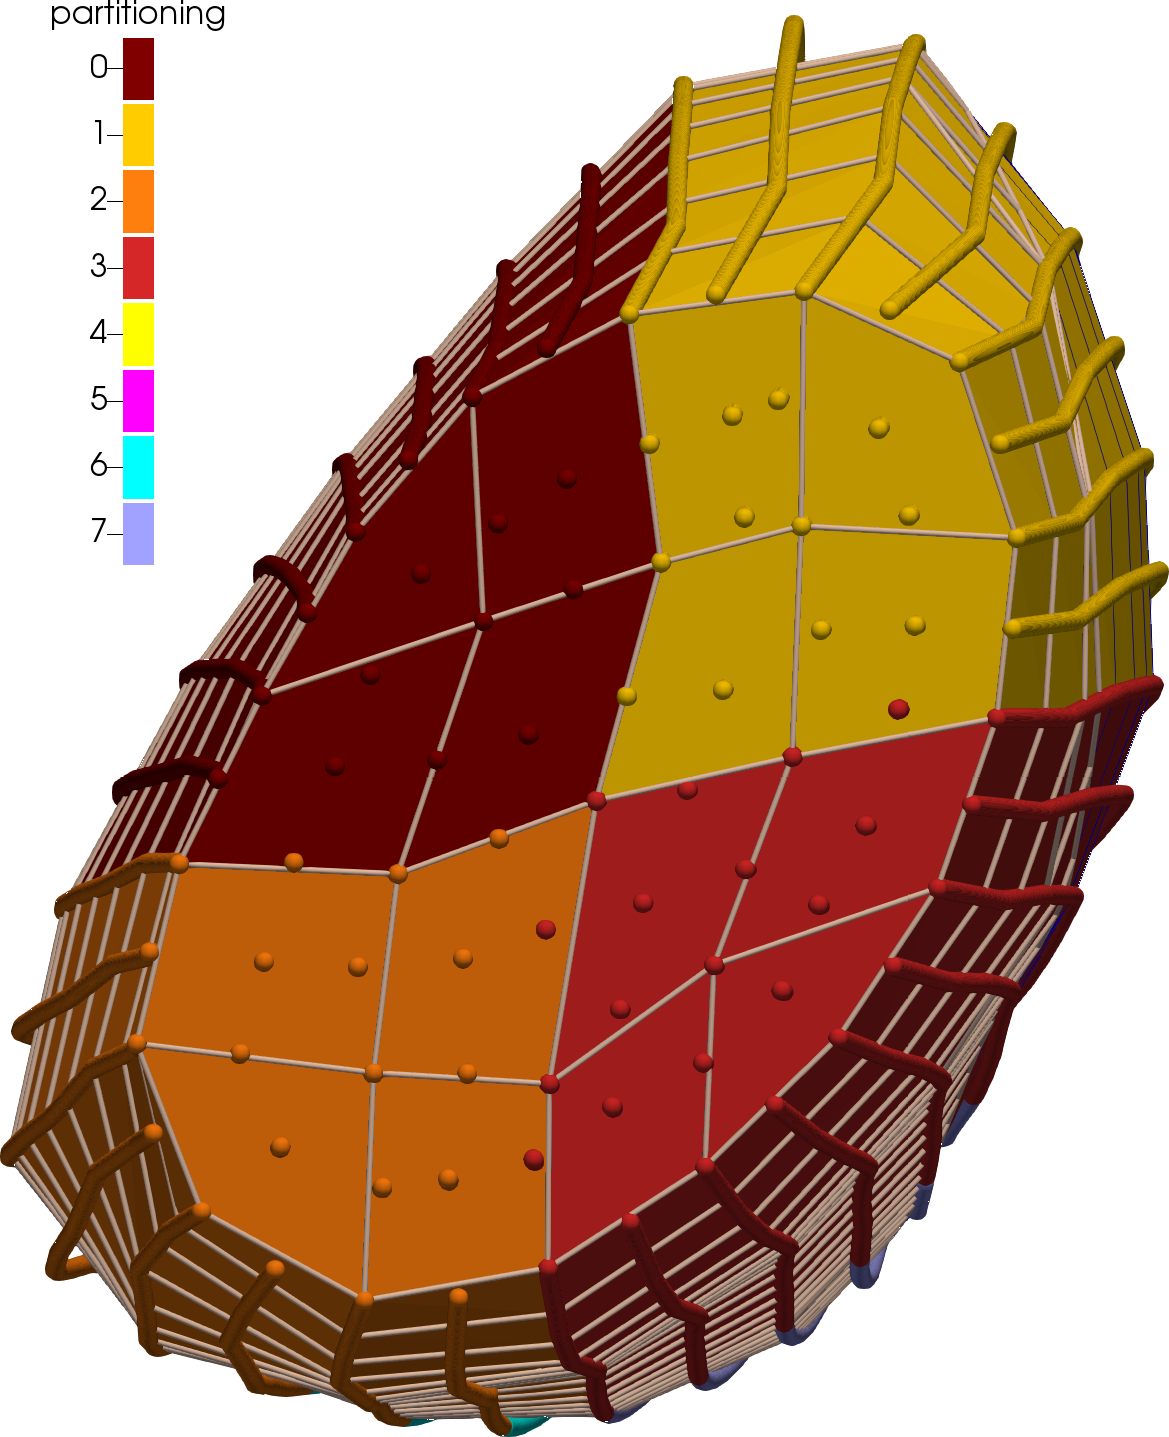
\includegraphics[width=\textwidth]{images/implementation/partitioning4.png}
    \caption{Resulting sampled mesh with option \code{distribute_nodes_equally=False}.}%
    \label{fig:partitioning4}%
  \end{subfigure}
  \quad
  \begin{subfigure}[t]{0.48\textwidth}%
    \centering%
    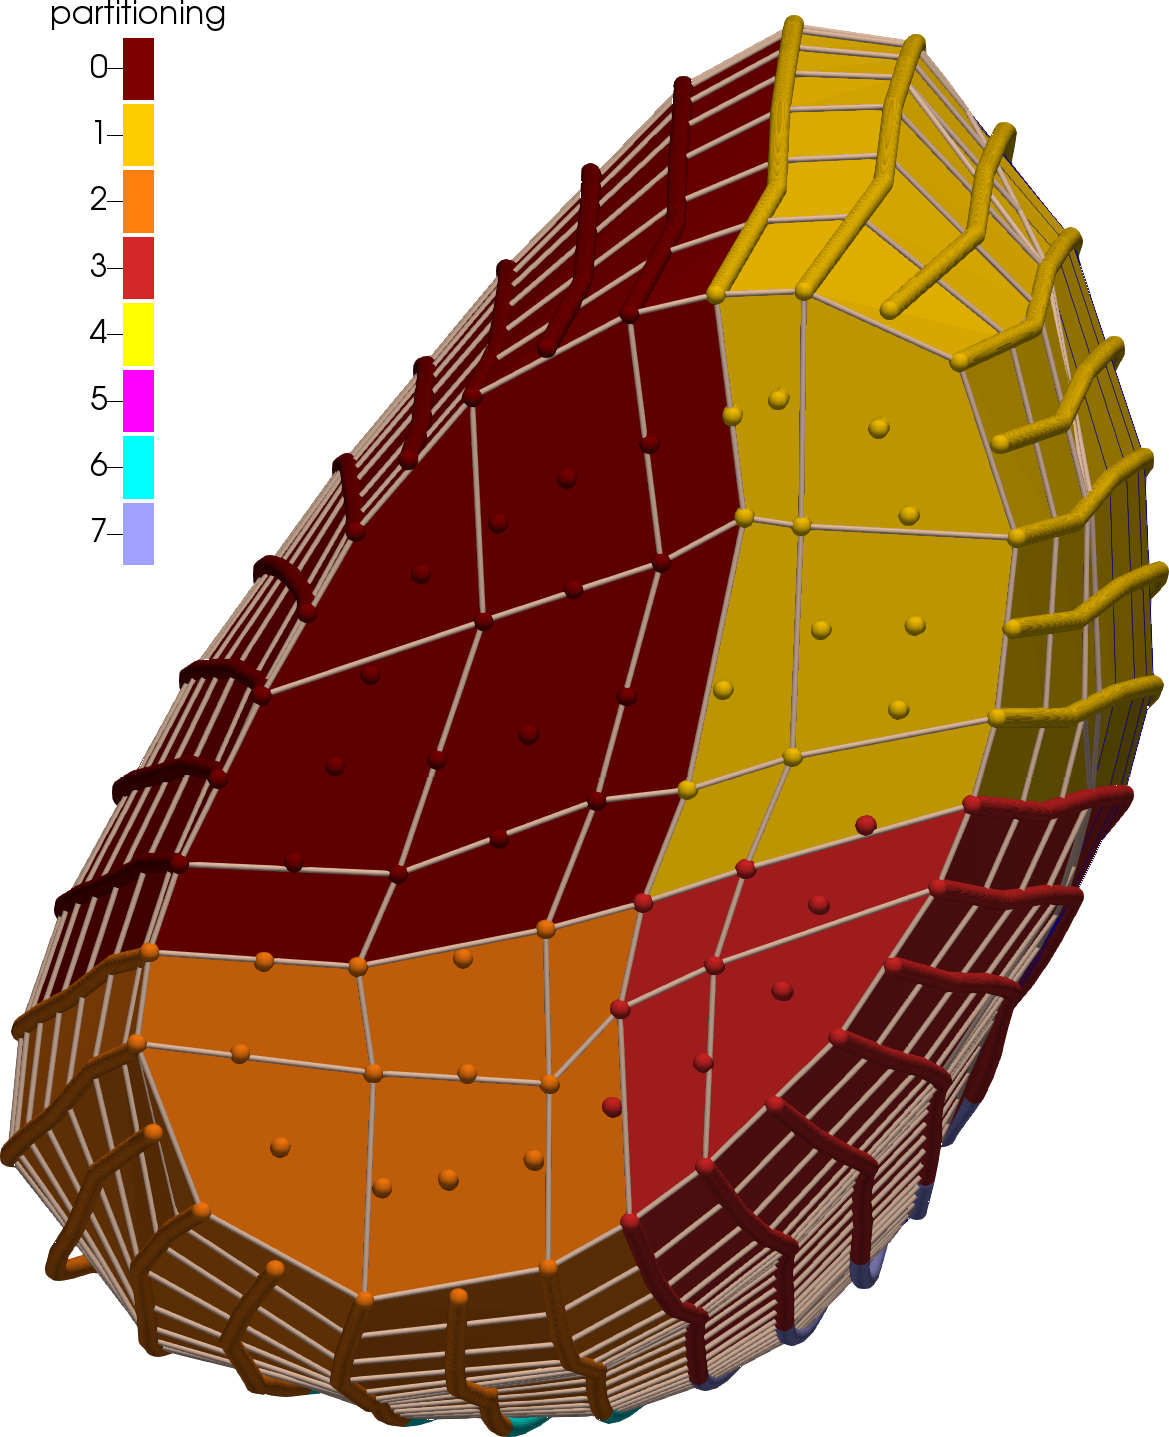
\includegraphics[width=\textwidth]{images/implementation/partitioning3.png}
    \caption{Resulting sampled mesh with option \code{distribute_nodes_equally=True}.}%
    \label{fig:partitioning3}%
  \end{subfigure}
  \caption{Mesh partitions generated by the sampling algorithm with different settings. A fine mesh with 49 fibers is sampled with a stride parameter of two and partitioned to eight processes.}%
  \label{fig:partitioning3_4}%
\end{figure}%

% partitioning with and without distribute_nodes_equally
\begin{figure}%
  \centering%
  \begin{subfigure}[t]{0.48\textwidth}%
    \centering%
    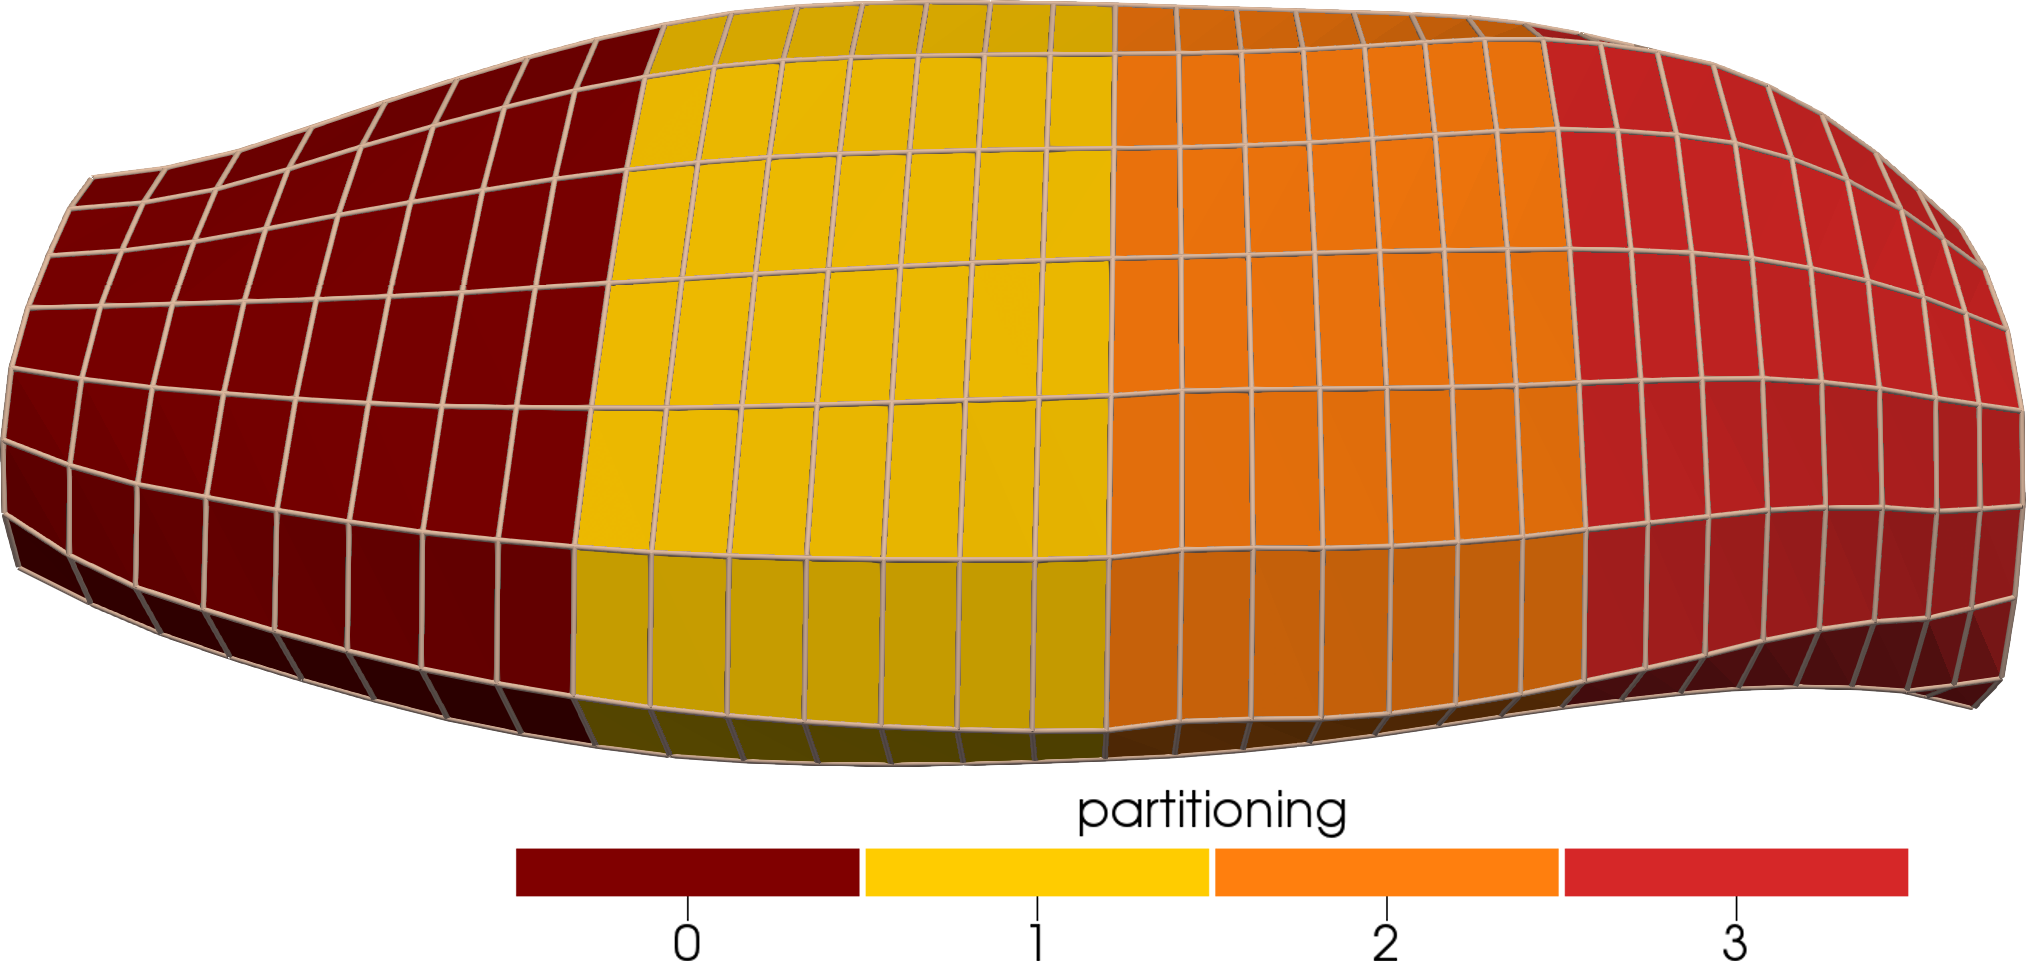
\includegraphics[width=\textwidth]{images/implementation/partitioning6.png}
    \caption{Resulting sampled mesh with option \code{distribute_nodes_equally=False}. The mesh width is constant, but the partitioning is not perfectly balanced.}%
    \label{fig:partitioning6}%
  \end{subfigure}
  \quad
  \begin{subfigure}[t]{0.48\textwidth}%
    \centering%
    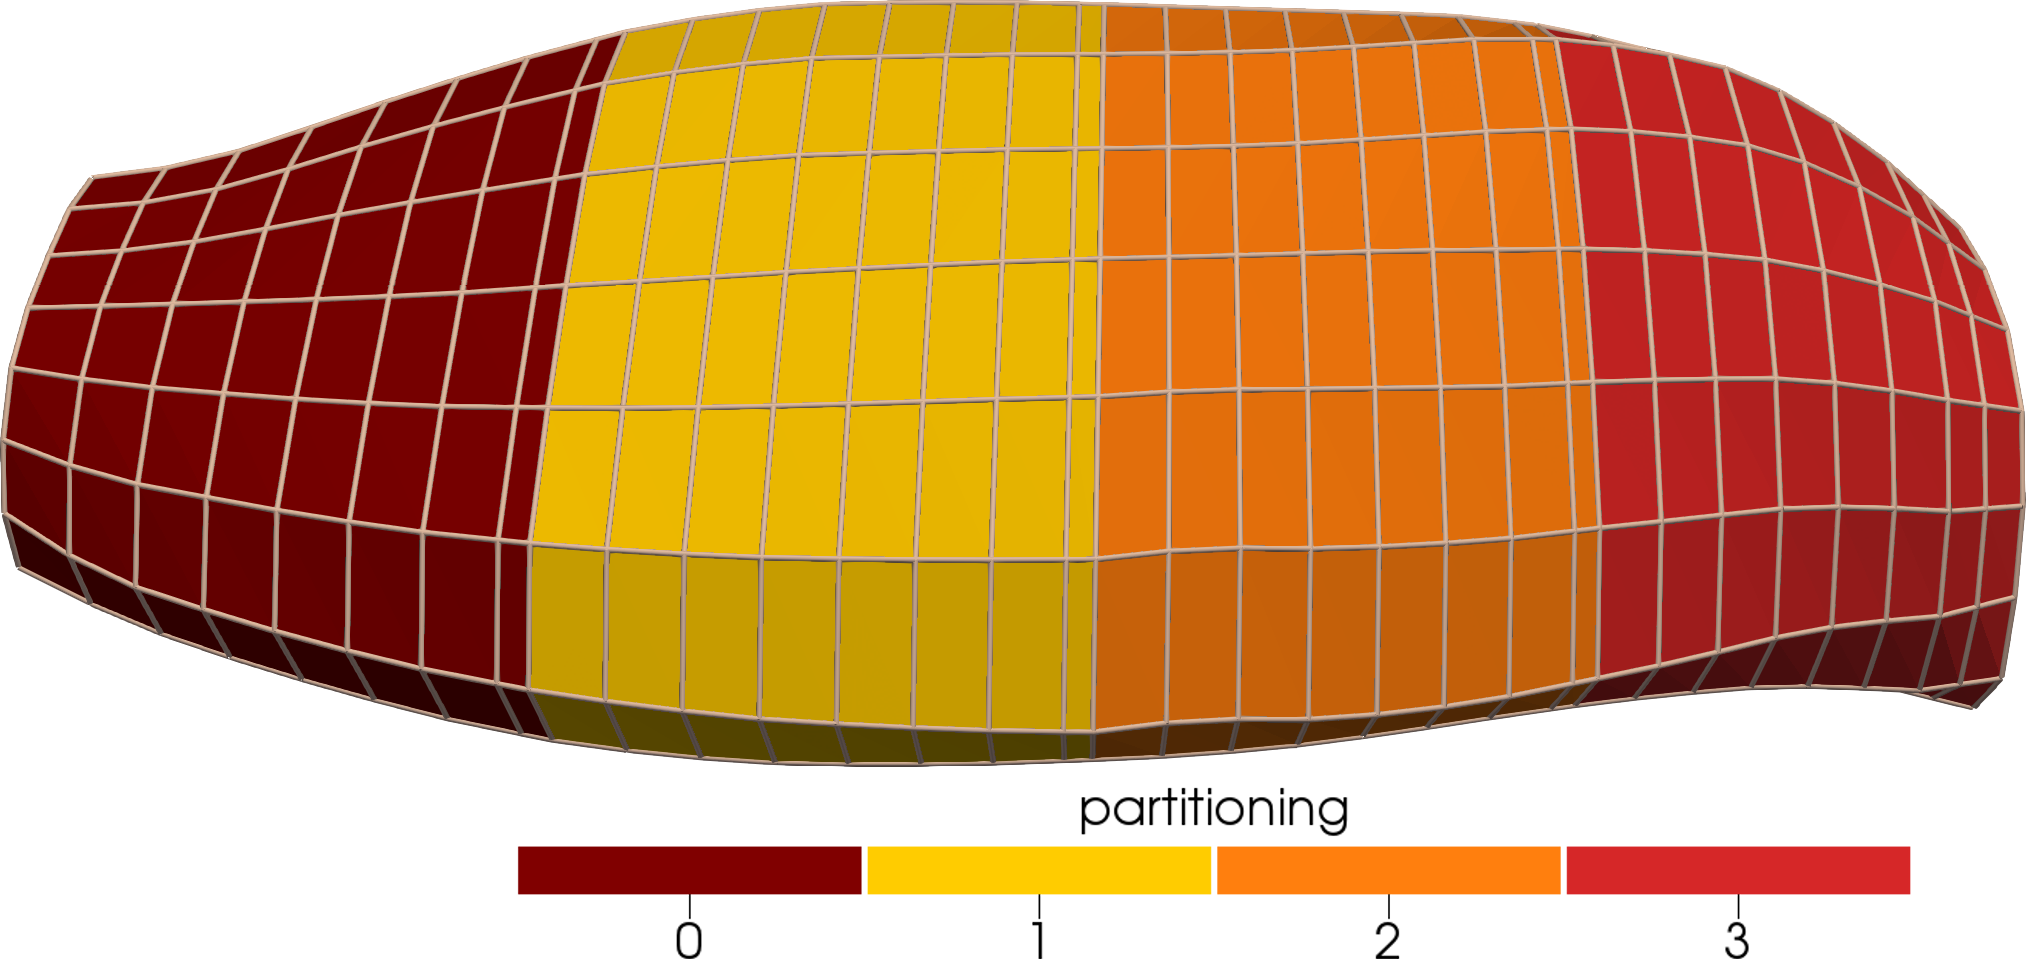
\includegraphics[width=\textwidth]{images/implementation/partitioning5.png}
    \caption{Resulting sampled mesh with option \code{distribute_nodes_equally=True}. The partitioning is perfectly balanced, but the mesh width is not constant.}%
    \label{fig:partitioning5}%
  \end{subfigure}
  \caption{Sampling a mesh along the fiber direction. The original mesh has 1481 nodes and is sampled with a stride value of 50.}%
  \label{fig:partitioning56}%
\end{figure}%


\begin{reproduce_no_break}
  The partitioning in \cref{fig:partitioning1} is obtained by the following simulation:
  \begin{lstlisting}[columns=fullflexible,breaklines=true,postbreak=\mbox{\textcolor{gray}{$\hookrightarrow$}\space}]
    cd $\$$OPENDIHU_HOME/examples/electrophysiology/fibers/fibers_contraction/no_precice/build_release
    mpirun -n 12 ./biceps_contraction ../settings_biceps_contraction.py partitioning_demo.py --n_subdomains 4 3 1
  \end{lstlisting}
  The partitionings in \cref{fig:partitioning3_4,fig:partitioning56} are created by the following simulations. For \cref{fig:partitioning4,fig:partitioning6}, edit the variables file \code{partitioning_demo.py} and set \code{distribute_nodes_equally = False}. For \cref{fig:partitioning3,fig:partitioning5}, set \code{distribute_}\code{nodes_equally = True}.
  \begin{lstlisting}[columns=fullflexible,breaklines=true,postbreak=\mbox{\textcolor{gray}{$\hookrightarrow$}\space}]
    cd $\$$OPENDIHU_HOME/examples/electrophysiology/fibers/fibers_emg/build_release
    mpirun -n 8 ./fast_fibers_emg ../settings_fibers_emg.py partitioning_demo.py
    mpirun -n 4 ./fast_fibers_emg ../settings_fibers_emg.py partitioning_demo.py --n_subdomains 1 1 4
  \end{lstlisting}
\end{reproduce_no_break}


\section{Parallel Solver for the Fiber Based Electrophysiology Model}\label{sec:parallel_partitioning_for_fiber_based}

After discussing the general partitioning and sampling of 3D and 1D meshes in the last section, we now focus on the concrete application for the fiber based electrophysiology model.
\Cref{sec:parallel_partitioning_for_fiber_based_solver} begins with a description of the solver structure and the parallelization. Subsequently, performance improvements considering the parallel execution of the solver are discussed. \Cref{sec:improved_parallel_solver_for_fiber_based} presents a variant, where a faster solver is employed for the 1D part of the computation. \Cref{sec:adaptive_computation_for_fiber_based} shows how the computational load can be reduced by only computing activated parts of the muscle.

\subsection{Parallel Solver Structure}\label{sec:parallel_partitioning_for_fiber_based_solver}
For better visualization, we consider the 2D setting of a mesh and embedded 1D fibers partitioned to $2\times 2$ processes as shown in \cref{fig:mesh_structure} by different colors. However, all discussions are also valid for the real 3D setting shown in the last section and for abitrary partitionings to $n_x \times n_y \times n_z$ processes.

% program structure and partitioning
\begin{figure}%
  \centering%
  \begin{subfigure}[t]{0.30\textwidth}%
    \centering%
    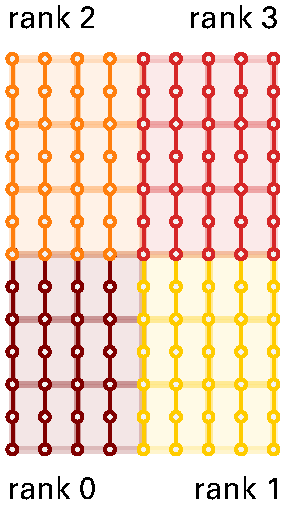
\includegraphics[width=\textwidth]{images/implementation/mesh_structure.pdf}
    \caption{Visualization of the 3D mesh with embedded 1D fibers, partitioned to four ranks.}%
    \label{fig:mesh_structure}%
  \end{subfigure}
  \qquad
  \begin{subfigure}[t]{0.45\textwidth}%
    \centering%
    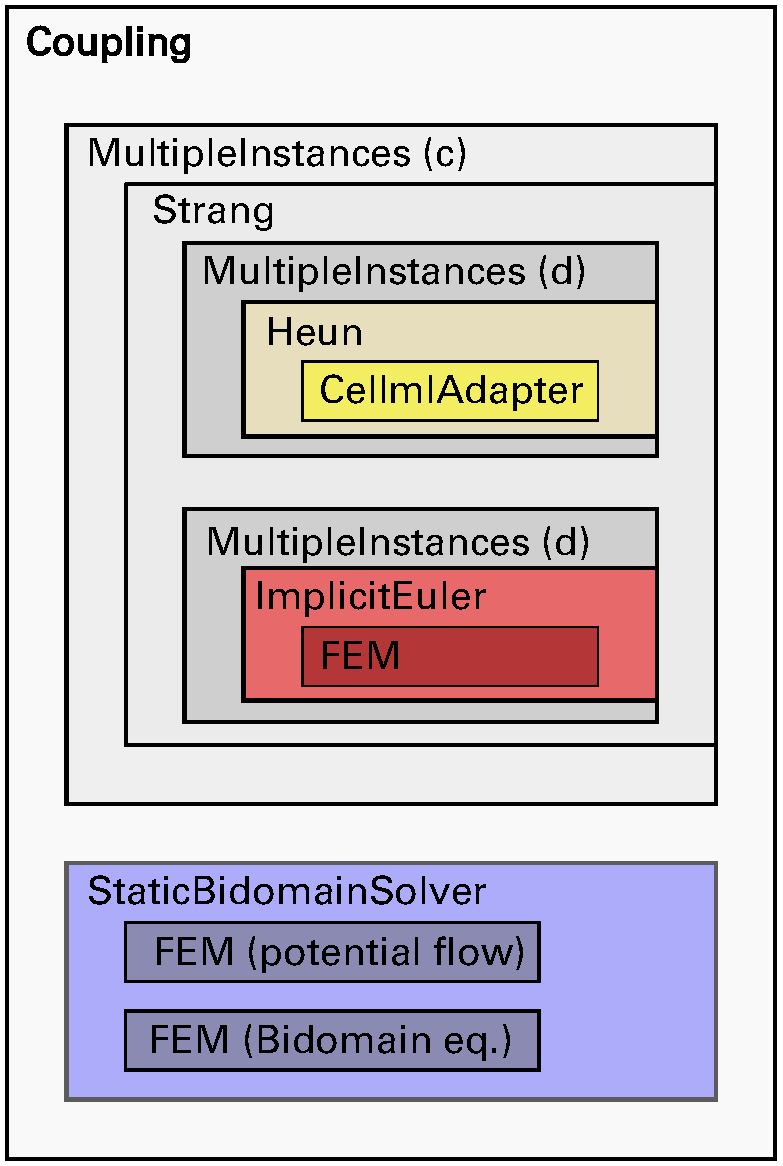
\includegraphics[width=\textwidth]{images/implementation/program_structure.pdf}
    \caption{Structure of the OpenDiHu example program to solve the fiber based electrophysiology model.}%
    \label{fig:program_structure}%
  \end{subfigure}
  \\[8mm]
  \begin{subfigure}[t]{0.48\textwidth}%
    \centering%
    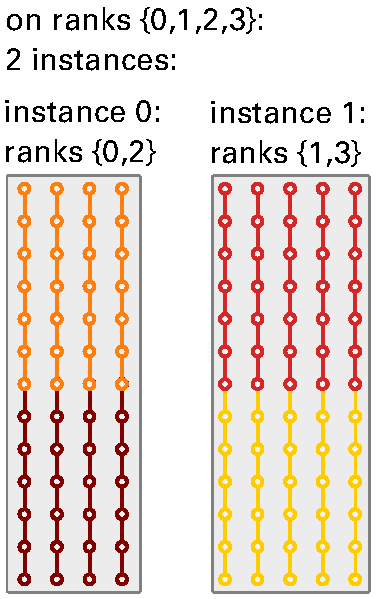
\includegraphics[height=8cm]{images/implementation/fiber_partitioning1.pdf}
    \caption{Instances of the outer \code{MultipleInstances} class in \cref{fig:program_structure}.}%
    \label{fig:fiber_partitioning1}%
  \end{subfigure}
  \,
  \begin{subfigure}[t]{0.48\textwidth}%
    \centering%
    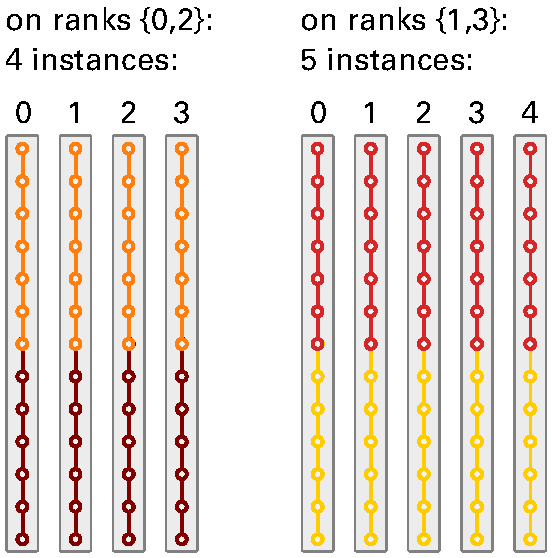
\includegraphics[height=7.5cm]{images/implementation/fiber_partitioning2.pdf}
    \caption{Instances of the inner \break\code{MultipleInstances} classes in \cref{fig:program_structure}.}%
    \label{fig:fiber_partitioning2}%
  \end{subfigure}
  \caption{Visualizations for the discussion of the program structure and partitioning used for fiber based electrophysiology simulations.}%
  \label{fig:partitioning_program}%
\end{figure}%

\Cref{fig:program_structure} shows the program structure of the example that solves the fiber based electrophysiology model. The outer class is a \code{Coupling} that alternates between computing the monodomain equation on the 1D fibers and computing the static bidomain equation on the 3D domain. The second part, the bidomain solver, is given in \cref{fig:program_structure} by the class \code{StaticBidomainSolver}, which includes two \code{FiniteElementMethod} classes. The first class solves the potential flow to obtain the fiber direction for the anisotropic conduction tensor, the second class is used to discretize the spatial derivatives in the bidomain equation.

The first part of the coupling scheme in \cref{fig:program_structure} consists of a tree of a \code{Multiple}\code{Instances} class that encloses the Strang operator splitting. The splitting has two child solvers for the subcellular model and the diffusion or conduction term. The first child consists of another \code{MultipleInstances} class with a \code{Heun} scheme and the \code{CellmlAdapter}\nolinebreak.
The second child of the Strang splitting also consists of a \code{MultipleInstances} class and a combination of an \code{ImplicitEuler} scheme (alternatively a \code{CrankNicolson} scheme can be used) and a \code{FiniteElementMethod}.

A \code{MultipleInstances} class can be used to apply a solver to more than one problem of the same kind. The class allows to specify a number of instances of its nested solver. Each instance can be given a subset of processes that will take part in the computation of the instance. Each process then iterates over all instances where it is part of the subset. Thus, the nested solver of a \code{MultipleInstances} class is called in series for all instances that share a process and it is called in parallel and independently for instances that have disjoint subsets of ranks.

Furthermore, the class provides a common output writer that collectively writes the data of all instances. This allows, e.g., to create a single output file in every timestep containing the data of all fibers. Especially for large scenarios, this is more practical than having as many output files as there are fibers.

The settings that have to be specified in the Python file for a \code{MultipleInstances} class comprise the number of instances and a list with the according number of entries, which further configure the instances. Each list entry can be \code{None} if the rank does not take part in the computation of the corresponding instance. 
Otherwise, the list entry consists of (i) a specification of all ranks that should collectively compute the corresponding instance and (ii) the settings of the corresponding nested solver. 

The own MPI rank of a process is known in the Python settings file. This allows to specify different settings for different ranks in the same file. By omitting the configuration of irrelevant instances and setting their list entry to \code{None}, the amount of data is reduced and parsing of the script is sped up, especially for large problem sizes.

The settings and corresponding subdomains of the \code{MultipleInstances} classes that are indicated by (c) and (d) in \cref{fig:program_structure} are shown in \cref{fig:fiber_partitioning1,fig:fiber_partitioning2}, respectively.
As can be seen in \cref{fig:fiber_partitioning1}, the outer \code{MultipleInstances} class separates the subdomains that are not connected by any fibers such that they can be computed in parallel and independently of each other. In the example of \cref{fig:mesh_structure}, the subdomains of ranks 0 and 2 can be computed independently of the subdomains of ranks 1 and 3. In consequence, all processes specify that their \code{MultipleInstances} class has two instances. At rank 0, the list of instance settings contains in the first list item the settings of the nested Strang solver with all information of rank 0's subdomain and in the second list item the value \code{None}, as rank 0 has no information about fibers outside of its subdomain. Ranks 1, 2 and 3 specify their subdomain accordingly, as shown in \cref{fig:fiber_partitioning1}.

During computation, ranks 0 and 2 as well as ranks 1 and 3 enter the \code{Strang} solver class collectively with a shared MPI communicator.
The inner \code{MultipleInstances} classes employ the 0D subcellular and 1D electric conduction solvers on multiple fibers. As shown in \cref{fig:fiber_partitioning2}, ranks 0 and 2 specify four instances with the settings of the four shared fibers. At the same time and concurrently, ranks 1 and 3 specify five instances with settings for their five shared fibers. 

Note that the multiplicity of the 0D instances on a fiber is not achieved by another \code{MultipleInstances} class but the model is solved for all points on the mesh together, using parallelism on the lower, instruction-based level.

These different splits of the geometry allow to compute the electrophysiology model on the fibers in parallel. The partitioning of the domain has to be the same for the 3D mesh and the embedded fibers to allow value mapping from the fibers to the 3D mesh without communication. The fibers are oriented along the $z$-direction in the 3D setting. This explains why the ranks for a particular fiber, e.g., $\{0,2\}$ or $\{1,3\}$ are not direct successors of each other but increasing with a stride equal to the number of subdomains in $x$ and $y$ directions, $n_x \cdot n_y$.

\subsection{Improved Parallel Solver Scheme using the Thomas Algorithm}\label{sec:improved_parallel_solver_for_fiber_based}
% FastMonodomainSolver

The monodomain model that is solved on each fiber consists of a reaction-diffusion equation that is solved using the Strang operator splitting.
The diffusion part uses an implicit timestepping scheme, which leads to a linear system of equation to be solved in every timestep.
As the Finite Element method with linear ansatz functions is used for spatial discretization, this linear system has a tridiagonal system matrix.

In the solver tree structure in \cref{fig:program_structure}, this solution step occurs in the solvers under the second inner \code{MultipleInstances} class.  As can be seen in \cref{fig:fiber_partitioning2}, the dofs of each fiber that are part of this linear system are partitioned to multiple processes. Hence, this linear system is solved using a parallel conjugate-gradient solver of PETSc.

However, there is the possibility to improve the performance by exploiting the tridiagonal matrix structure. The \emph{Thomas algorithm} is the specialization of Gaussian elemination for this matrix type and is known to efficiently solve such a system in linear time complexity. More specifically, it only requires a first downwards sweep through the matrix entries for forward substitution and a second upwards sweep for back substitution to compute the solution. It is stable for diagonally dominant matrices and this condition is met for the governing system matrix.

As the Thomas algorithm is not parallel, we have to gather the matrix data on a single process in order to employ the algorithm. In OpenDiHu, the \code{FastMonodomainSolver} class is taylored to the parallel solution of fiber based electrophysiology using the Thomas algorithm.
The parallel partitioning of the fibers is carried out normally, as described in \cref{sec:parallel_partitioning_for_fiber_based}. Before the computation, the fiber data in \cref{fig:fiber_partitioning2} are communicated such that every fiber is completely present at a single processes. The assignment of the fibers to processes occurs in a round-robin fashion, i.e., the first fiber is sent to rank 0, the second to the next rank, etc. In result, every process has approximately the same number of complete fibers. The processes then each compute the full monodomain model consisting of the Strang splitting with the subcellular model on the nodes of each fiber and the diffusion part using the Thomas algorithm.

In the C++ file, the \code{FastMonodomainSolver} class is inserted as a wrapper to the outer \code{MultipleInstances} class that is indicated by (c) in the solver structure in \cref{fig:mesh_structure}. In the Python settings, the class does not add an additional nesting level such that the same settings file can be used for programs with and without the \code{FastMonodomainSolver} class and yields the same simulation results.

During initialization, the \code{FastMonodomainSolver} class initializes its nested solver tree as normal. At the beginning of the first timestep, the communication to gather complete fiber data on single processes is carried out. Then, the monodomain equation is solved in a separate serial implementation for the now locally owned fibers, i.e., not using the nested solvers. The solution is obtained for as many subsequent timesteps as were specified in the settings. When the end time of the enclosing coupling scheme is reached, the fiber data is communicated back to the original partitioned fibers. Then, the coupling scheme continues with the data mapping from the partitioned fibers to the 3D domain and with the \code{StaticBidomainSolver}. Afterwards, the \code{FastMonodomainSolver} is called again and performs its computation anew starting with the communication step.

In summary, the efficient serial computation of the monodomain model in the \code{Fast}\code{MonodomainSolver} is wrapped by communication steps of  the partitioned fiber data. The frequency of this communication step is determined by the timestep width of the coupling scheme. 
The scenario solves the bidomain equation to simulate EMG signals. A typical sampling frequency of EMG capture devices is $f=\SI{2}{\kilo\hertz}$, which corresponds to a coupling timestep width of $\dt_\text{3D}=\SI{0.5}{\milli\second}$. The timestep widths $\dt_\text{0D}$ of the subcellular model and $\dt_\text{1D}$ of the diffusion term have to be set at maximum to $\SI{1e-3}{\milli\second}$, yielding \num{500} timesteps of computations on the fiber between subsequent communication steps. As a result, the communication cost is negligible.

\subsection{Adaptive Computation of the Subcellular Model}\label{sec:adaptive_computation_for_fiber_based}
% adaptive solution of cells and whole fibers

During simulations of the fiber based electrophysiology model, often only a small fraction of the given fibers are activated.
The reason is that in physiological conditions the smaller MUs are activated first and the larger MUs only get activated when the full force of the muscle is required. As the majority of the fibers belongs to larger MUs, a high portion of fibers is less frequently activated, also depending on the scenario.
But even if the scenario specifies a tetanic stimulation of all MUs, the larger MUs have lower stimulation frequencies which again leads to less action potentials on large MUs than on smaller MUs in the same time span.

A naive solver of the monodomain models always computes all 1D electric conduction problems on the fiber meshes and all 0D subcellular models on the nodes of the fiber meshes, regardless of their activation state. In the following, we present a method in OpenDiHu that exploits the infrequent activation events on most of the fibers while obtaining the same solution as the naive solver.

We assume that the subcellular models are initialized in their equilibrium state, where the temporal derivative of the state vector $\bfy$ vanishes, $∂\bfy/∂t = 0$. The first algorithmic improvement is to only consider those fibers in the solver that have yet been stimulated. This improves the performance especially for \say{ramp like} motor recruitment where more and larger MUs are activated over time. However, after all MUs have been activated at least once, all fibers are computed again and no more performance improvement is obtained.

The second improvement is to only compute instances of the subcellular model at those points where it is not in equilibrium. To determine if an instance of the subcellular model is in equilibrium, we compare the solution before and after one integration step by the Heun method. Only if the relative change of any component of the state vector $\bfy$ is larger than \num{1e-5}, we consider the model to be not in equilibrium.

This check requires to compute the solution of the subcellular model, the avoidance of which is subject of the improved scheme. Therefore, we use the property of the 1D diffusion problem discretized by linear Finite Elements that the value at one spatial point can only influence its two neighbors in a single timestep. This allows us to avoid checking the equilibrium condition at points that are surrounded by other points in equilibrium. This means that the subcellular model does not have to be solved at most points in equilibrium, which drastically reduces the runtime. The 1D electric conduction problem, however, has to be solved for the whole fiber mesh if at least one point one it is not in equilibrium.

In our method, each subcellular point can be in one of the three states \say{active}, \say{inactive} and \say{neighbor is active}.
If the subcellular model is not in equilibrium, the point is in the state \say{active} and has to be solved in the next timestep. If the subcellular model is in equilibrium and does not have to be solved because the solution vector stays constant, the point is in the state \say{inactive}. The state \say{neighbor is active} occurs for a previously inactive point, of which at least one neighbor became active and, thus, the check if the point is still in equilibrium has to be performed and the subcellular model has to be solved in the next timestep. After each solution step, the state of a point changes according to the transitions given in \cref{fig:state_chart}.

An active point stays active, if the solution has changed in the last numeric integration step. It transitions to inactive, if the solution did not change. The same applies to points in the state \say{neighbor is active}, which also change to \say{active} or \say{inactive} after one time step. 
An inactive state cannot be activated by a check on the point itself, as this state implies that no computation and subsequent equilibrium check are carried out. The only transition for a point $A$ from an inactive state occurs when a neighbor point $B$ reaches the state \say{active}. Then, point $A$ changes to \say{neighbor is active}.
For propagating action potentials along a fiber that is in the \say{inactive} state, this leads to a propagating front of points in the \say{neighbor is active} state.

Initially, all states are set to \say{active}. If no stimulation occurs and the subcellular model is in equilibrium, they momentarily change to \say{inactive}. Upon external stimulation, the stimulated points are automatically set to \say{active} and their neighbors are set to \say{neighbor is active} such that the effect of the stimulation can be considered in subcellular model computations.

% compute state
\begin{figure}%
  \centering%
  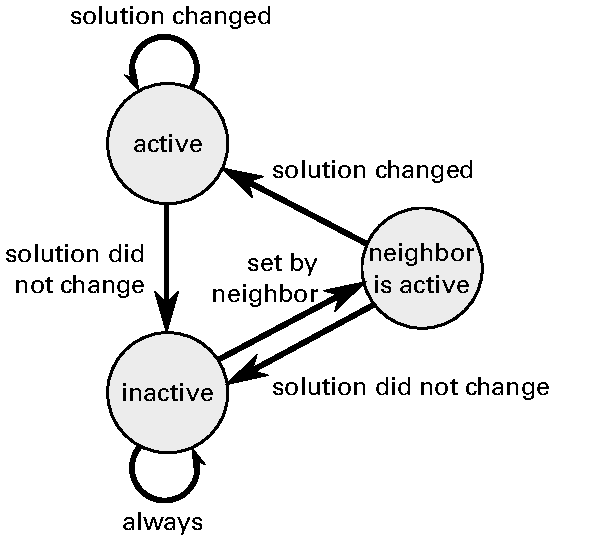
\includegraphics[width=0.6\textwidth]{images/implementation/state_chart.pdf}%
  \caption{Transition diagram for the adaptive computation of the subcellular model.}%
  \label{fig:state_chart}%
\end{figure}%

\Cref{fig:compute_state3} shows a simulation where the effect of both improvements are visible. The Hodgkin-Huxley subcellular model has been solved on a set of 49 fibers. At the displayed time of $t=\SI{28}{\milli\second}$, two MUs have been activated. The value of the membrane potential $V_m$ is visualized by the radius of the fibers. The active or inactive state of the improved scheme is indicated by the colors.

% compute state
\begin{figure}%
  \centering%
  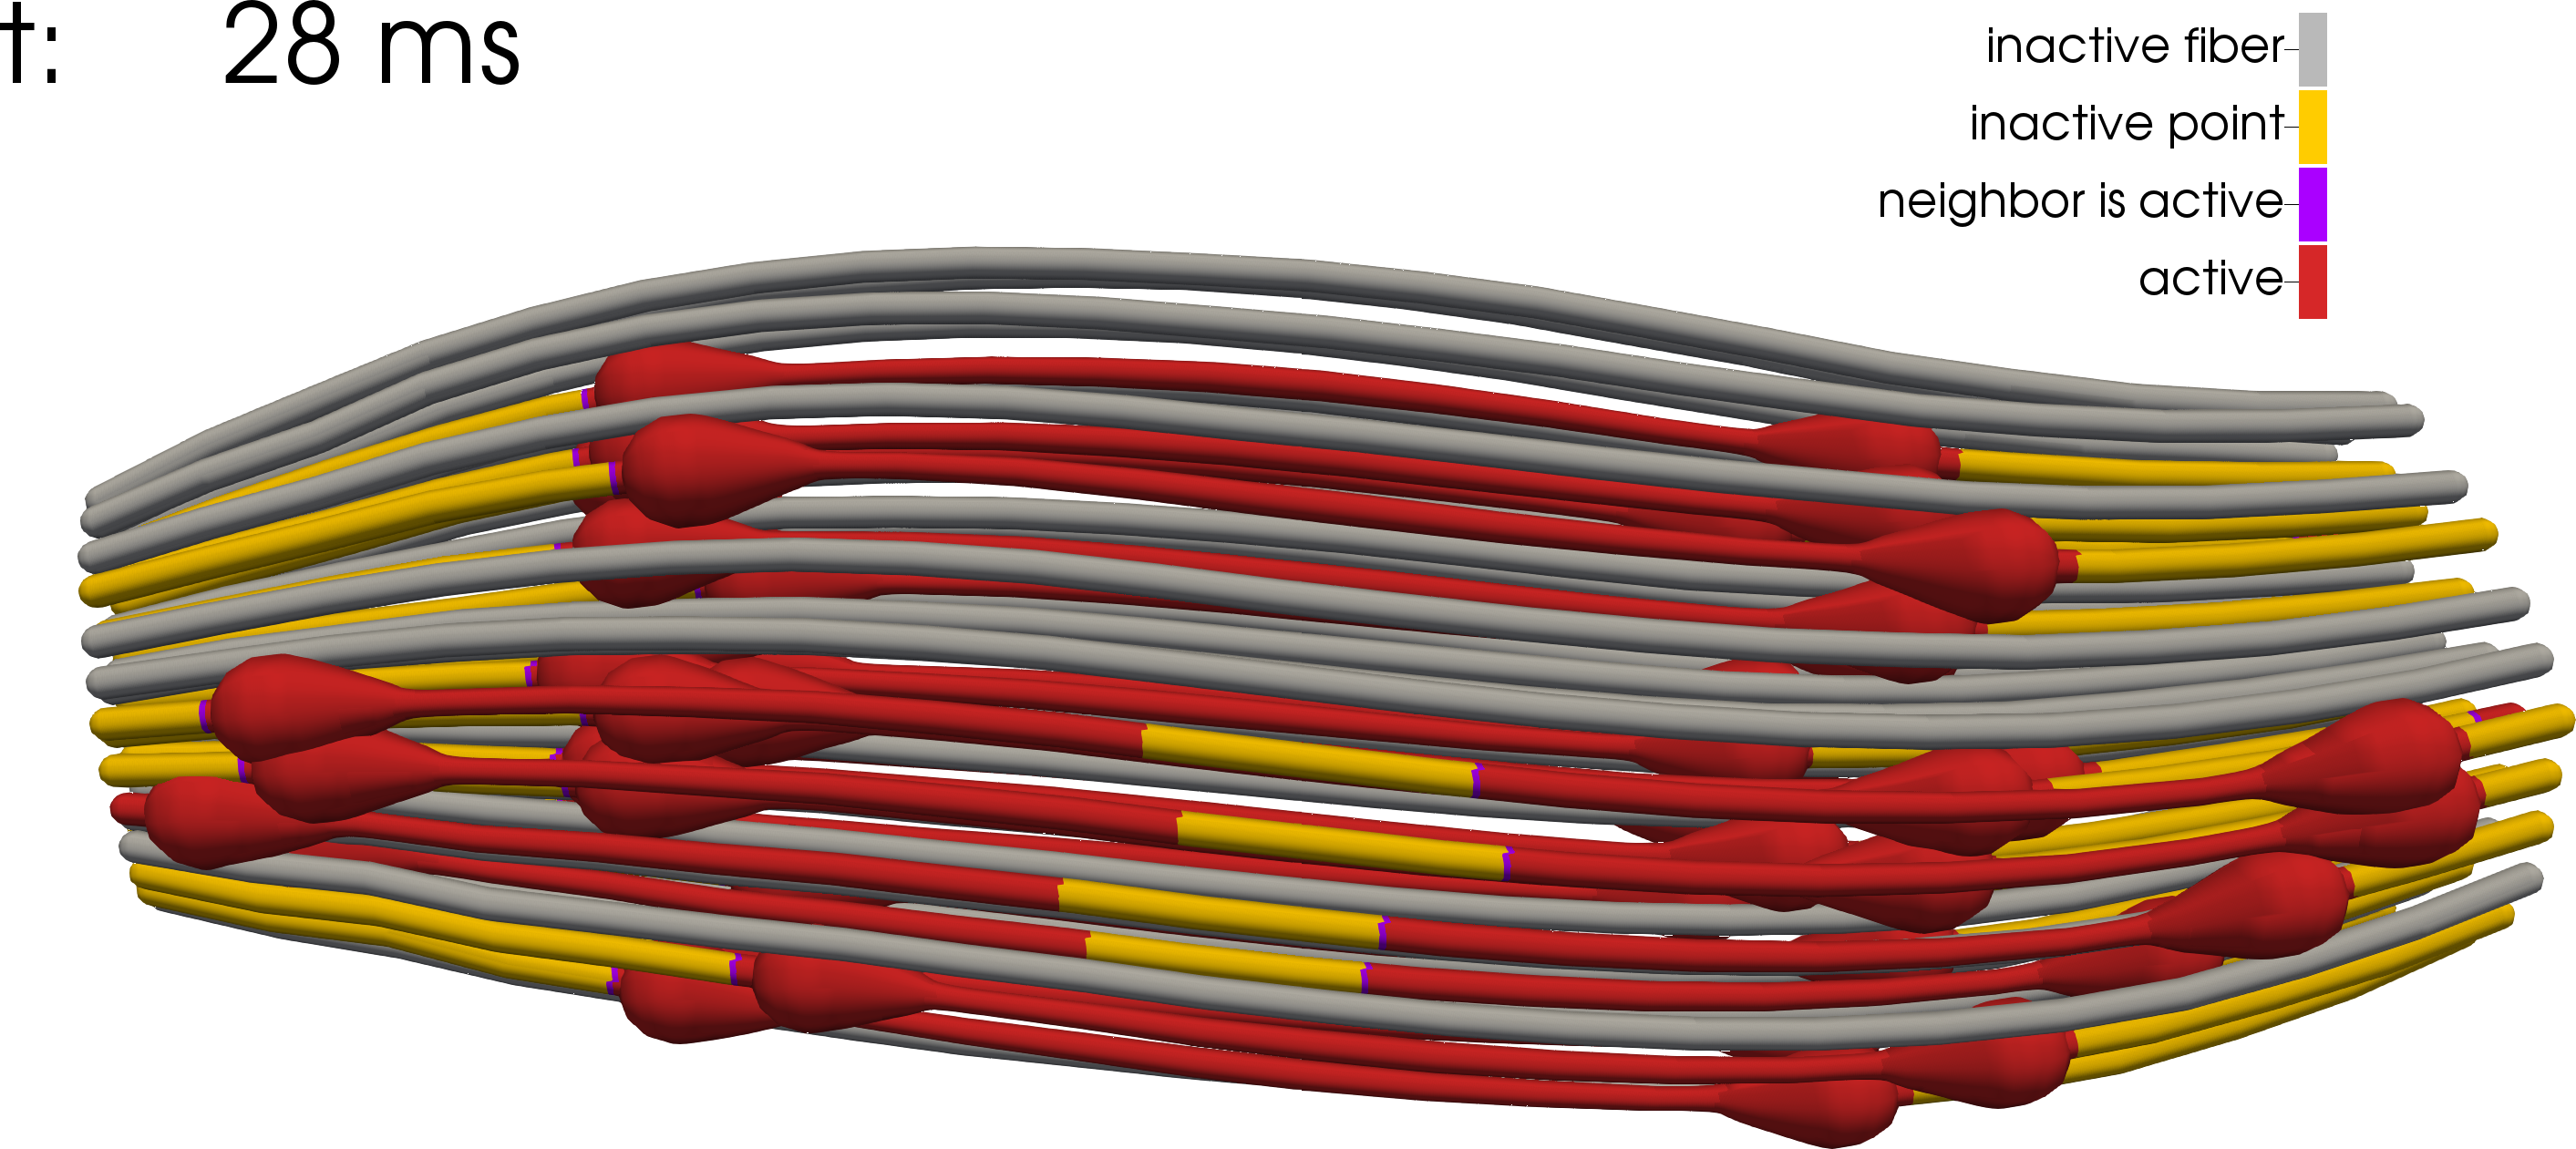
\includegraphics[width=\textwidth]{images/implementation/compute_state3.png}%
  \caption{Simulation scenario that demonstrates the adaptive computation method of fibers and subcellular points. A simulation of the monodomain equation on a set of 49 fibers with the subcellular model of Hodgkin and Huxley is shown. The transmembrane potential is visualized by the fiber radius. The states of the points used in the algorithm are given by the different colors.}%
  \label{fig:compute_state3}%
\end{figure}%

It can be seen that several fibers have gray color which indicates that they have not yet been stimulated and, thus, are not part of the computation. The other fibers have been stimulated either by the first or the second MU. Action potentials at two different distances from the center corresponding to the two MUs can be identified by the bulbous shapes. The red parts of the fibers contain the active points where the subcellular model is not in equilibrium. At the yellow regions, the subcellular models are in equilibrium and no computational work is performed there. The yellow regions are at the outer ends of the fibers that were not yet reached by the action potentials as well as around the center for fibers of the first MU. This demonstrates the repolarisation effect after which the model reaches its equilibrium state again. 

The purple colored points are in the state \say{neighbor is active} and can be found between active and inactive points. As the algorithm iterates over all points of a fiber from left to right, these purple points only occur at the left boundaries of active regions. At their right boundaries, the initial \say{neighbor is active} points transition to \say{active} or \say{inactive} directly after the computation step within this iteration.

Instead of individual nodes on the fiber mesh, our implementation treats SIMD vectors of four or eight such adjacent nodes (depending on the hardware capabilities) as one point in the algorithm.  If one of these nodal instances is not in equilibrium, the whole SIMD vector is considered not in equilibrium and transitions to the \say{active} state. This coarser granularity of the model instances allows to solve the subcellular problem in chunks according to the SIMD lane width using SIMD instructions.

\begin{reproduce_no_break}
  The scenario of \cref{fig:compute_state3} can be run as follows:
  \begin{lstlisting}[columns=fullflexible,breaklines=true,postbreak=\mbox{\textcolor{gray}{$\hookrightarrow$}\space}]
    cd $\$$OPENDIHU_HOME/examples/electrophysiology/fibers/fibers_emg/build_release
    mpirun -n 4 ./fast_fibers_emg ../settings_fibers_emg.py compute_state_demo.py
  \end{lstlisting}
  Instead of four processors you can use as many as you have to speed up the computation.
\end{reproduce_no_break}
\section{Parallel Solver for the Multidomain Electrophysiology Model}\label{sec:parallel_solver_multidomain}

After the details on the parallel partitioning and solvers for the fiber based electrophysiology model have been discussed in \cref{sec:parallel_partitioning_and_sampling_of_the,sec:parallel_partitioning_for_fiber_based}, we now consider the multidomain based model of electrophysiology, which includes electric conduction in the body fat layer. The class for the implicit solver within the operator splitting is the \code{MultidomainWithFatSolver} class, which has been introduced in \cref{sec:exemplary_usage_2}.

\subsection{Construction and Partitioning of the Mesh}

The mesh used in this solver is a composite mesh of type \code{Mesh::CompositeOfDimension<D>}, as introduced in \cref{sec:composite_meshes}. \Cref{fig:structured_grid_n_nodes} shows the layout how the mesh of the body fat domain $\Omega_B$ is connected with the mesh of the muscle domain $\Omega_M$. The muscle and body meshes have $N_x^\text{el} \times N_y^\text{el} \times N_z^\text{el}$ and $(N_x^\text{el}+ N_y^\text{el}) \times N_\text{fat}^\text{el} \times N_z^\text{el}$ elements, respectively. Only the muscle mesh has been generated from medical imaging data by the pipline given in \cref{sec:generation_of_meshes_for_multiscale}. The fat mesh is created on top of the muscle mesh geometry and has to use the same number of elements as the muscle mesh for compatibility in the composite mesh. Only the physical thickness of the adipose tissue layer and the corresponding number $N_\text{fat}^\text{el}$ of elements in radial direction have to be specified.  (The mesh generation step is implemented in the script \code{create_fat_layer.py}.) 

% fat layer mesh and partitioning
\begin{figure}
  \centering%
  \def\svgwidth{0.6\textwidth}
  \input{images/implementation/structured_grid_n_nodes.pdf_tex}%
  \caption{Layout of the composite 3D mesh for the multidomain model with fat layer. The orange elements belong to the mesh of the muscle domain $\Omega_M$, the yellow elements are added on top to represent the body domain $\Omega_B$.}%
  \label{fig:structured_grid_n_nodes}%
\end{figure}%

\Cref{fig:multidomain_matrix_mesh} shows such as composite mesh.
The muscle mesh is based on a dataset of $13\times 13$ fibers with \num{1481} nodes per fiber. This fine mesh is sampled as described in \cref{sec:algorithm_for_partitioning_and_sampling} with stride values of $3,3$ and $20$ in $x,y$ and $z$ directions and \code{distribute_nodes}\code{_equally=True}. In result, we get $N_x^\text{el} \times N_y^\text{el} \times N_z^\text{el} = 5 \times 4 \times 75$ elements.
The fat mesh consists of a $\SI{1}{\centi\meter}$ adipose tissue layer with $N_\text{fat}^\text{el}=4$ elements. The muscle and fat meshes have \num{2280} and \num{3800} dofs, yielding a 

% comment about parallelization
The partitioning of the composite mesh into $n_x \times n_y \times n_z$ subdomains cannot be chosen arbitrarily. The reason is that both the muscle and the body fat mesh have to be partitioned to the same number of processes. 
If, e.g., a partitioning of $n_x=n_y=2$ is chosen, the cube in \cref{fig:structured_grid_n_nodes} gets divided by one horizontal planar cut and one vertical planar cut. This divides the orange muscle mesh into four subdomains as expected. The yellow body fat mesh, however, is only partitioned to three of the four processes as there are no yellow elements below the horizontal cut and left of the vertical cut.

Thus, a valid partitioning can only be created if either $n_x$ or $n_y$ is set to one. Because there is no restriction on $n_z$, the total mesh can still be partitioned in two dimensions to a product of subdomains, either as $1 \times n_y \times n_z$ or as $n_x \times 1 \times n_z$.
The example mesh in \cref{fig:multidomain_matrix_mesh} is partitioned to $2 \times 1 \times 2$ subdomains as shown by the different colors.

% scenario_name: matrix,  n_subdomains: 2 1 2,  n_ranks: 4,  end_time: 0.002
% dt_0D:           1e-03    multidomain solver:         1000 it. of gmres (10000 it. of gmres), lumped mass matrix: False, initial guess: previous solution
% dt_multidomain:  1e-03    multidomain preconditioner: euclid (euclid), symmetric precond.: True
% dt_splitting:    1e-03    theta: 1.0, solver tolerances, abs: 1e-15, rel: 1e-15
% fiber_file:              ../../../input/left_biceps_brachii_13x13fibers.bin
% fat_mesh_file:           ../../../input/left_biceps_brachii_13x13fibers.bin_fat.bin
% cellml_file:             ../../../input/hodgkin_huxley_1952.c
% firing_times_file:       ../../../input/MU_firing_times_always.txt
% ********************************************************************************
% 4 ranks, partitioning: x2 x y1 x z2
%   sampling 3D mesh with stride 3 x 3 x 20 
%   distribute_nodes_equally: True
%     linear 3D mesh    nodes global: 6 x 5 x 76 = 2280, local: 3 x 5 x 38 = 570
%     linear 3D mesh elements global: 5 x 4 x 75 = 1500, local: 3 x 4 x 38 = 456
%     fat mesh, n points total:    3800 (10 x 5 x 76), (per process: 3 x 5 x 38 = 570)
% 
\begin{figure}
  \centering%
  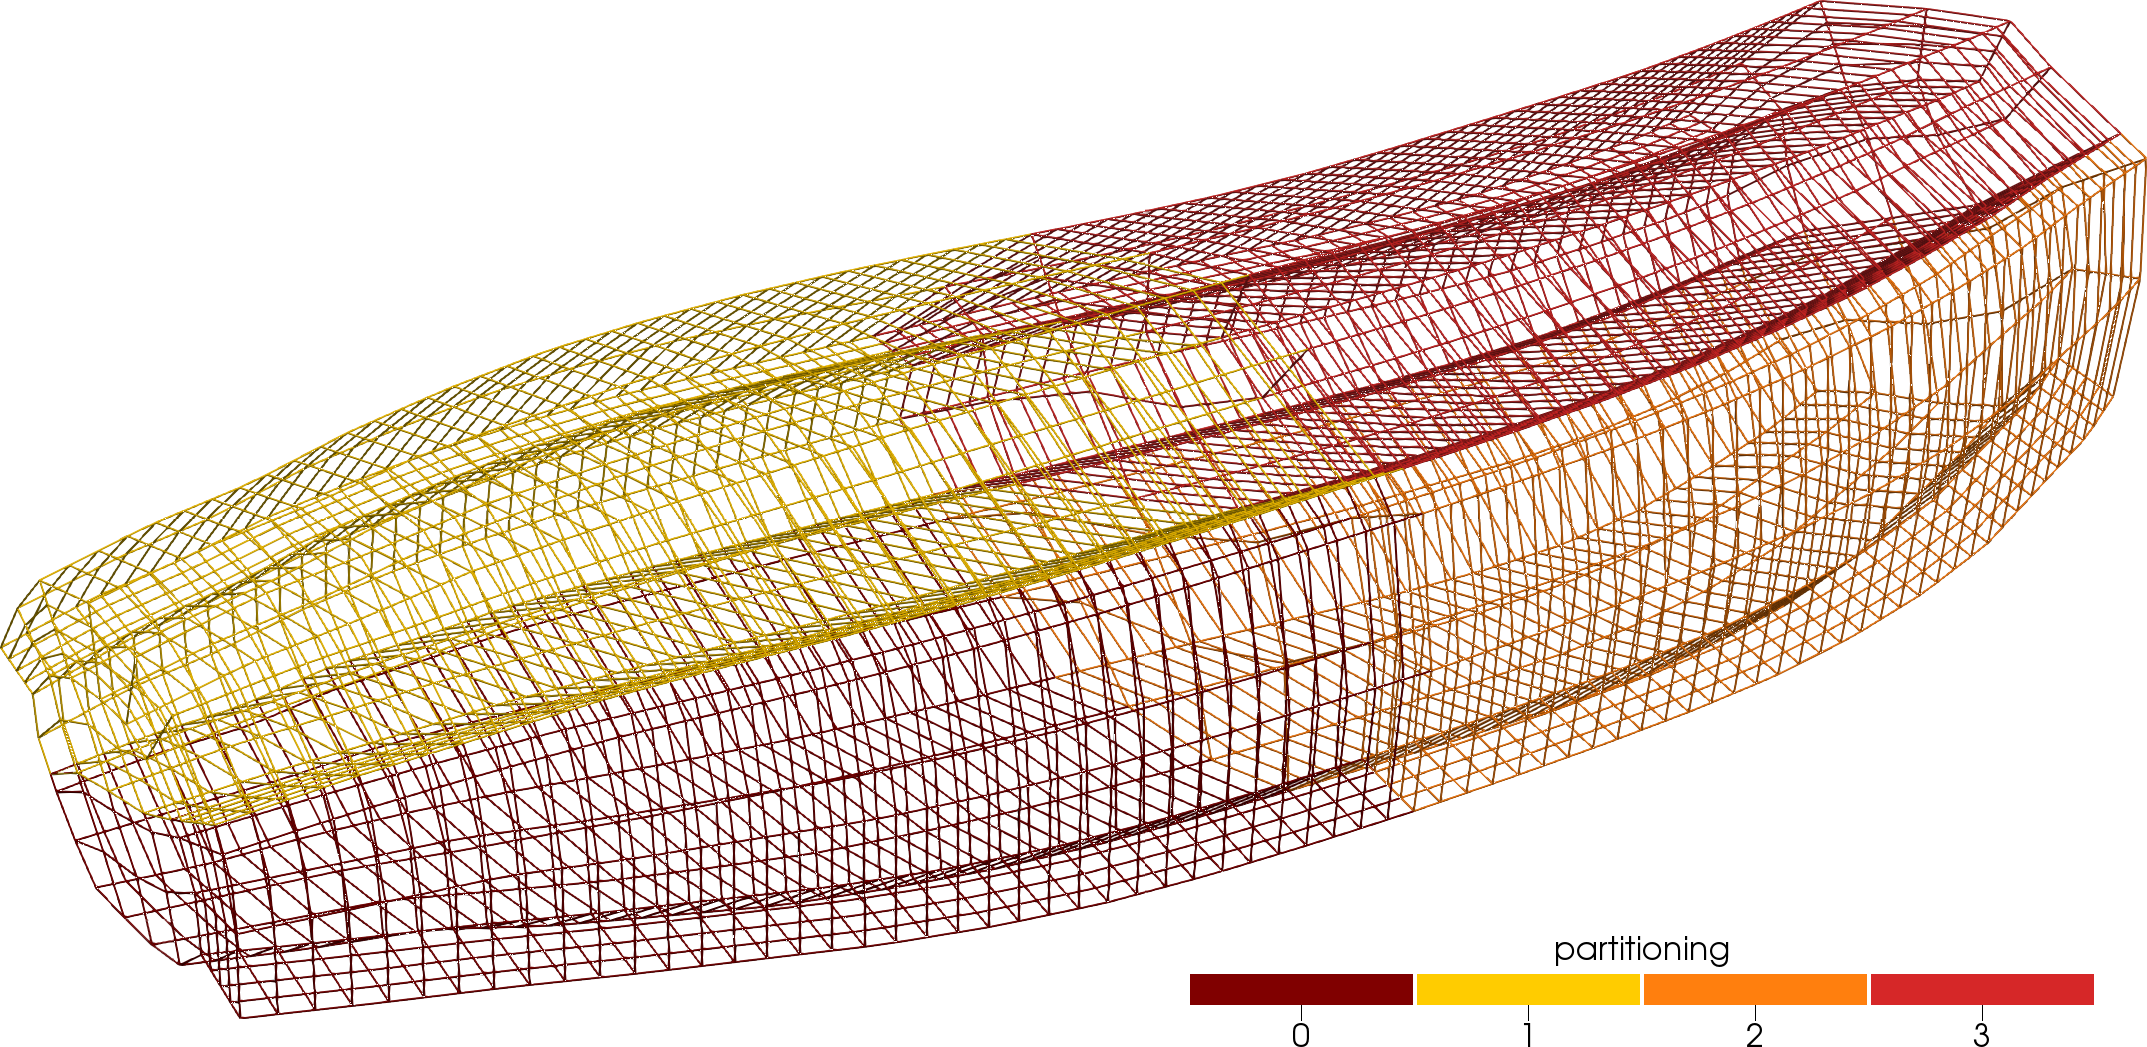
\includegraphics[width=\textwidth]{images/implementation/multidomain_matrix_mesh.png}%
  \caption{Composite mesh of the multidomain example, partitioned to four processes.}%
  \label{fig:multidomain_matrix_mesh}%
\end{figure}%

\subsection{Structure of the System Matrix}

The \code{MultidomainWithFatSolver} class uses nested \code{FiniteElementMethod} classes to describe the anisotropic electric conduction in the muscle domain and the isotropic electric conduction in the fat domain.
The system matrix for the system of equations is given in \cref{eq:discretized_multidomain_body2} in \cref{sec:discretization_body_domain}. 
The solver calculates the matrix block entries using the stiffness and mass matrices computed by the nested \code{FiniteElementMethod} classes.

\Cref{fig:original_matrix} shows the location of non-zeros in the resulting sparse matrix for three MUs. The matrix blocks are indicated by boxes and can be identified by comparison with \cref{eq:discretized_multidomain_body2}. In this visualization, it may seem that most of the blocks only have three non-zero entries per row, however, the actual number is higher with a maximum of 27 entries, as the Finite Element ansatz function of a node in the 3D mesh has overlapping support with the ansatz functions of other nodes in a $3\times 3 \times 3$ grid.
The actual non-zero structure per block is close to the example shown in \cref{fig:sparsity_pattern}.

The colors in \cref{fig:original_matrix} correspond to the four processes, as defined in the partitioned mesh in \cref{fig:multidomain_matrix_mesh}. 
The entries in every block are all partitioned in the same way to the four processes, as given by the partitioning of the nested \code{FiniteElementMethod} classes. The data structure for this layout is the \code{MATNEST} type of PETSc. 

However, to be able to apply the multitude of PETSc solvers to this linear system, the matrix has to be transferred to the canonical parallel matrix layout of PETSc that groups all dofs of the subdomains together. As this conversion is not available in PETSc, it is done in OpenDiHu by reordering the dofs and, in consequence, the matrix entries. The same permutation is applied to the rows and the columns of the matrix. The result of this operation is shown in \cref{fig:reordered_matrix}. It can be seen that the portions for each process are now consecutive matrix rows. The non-zero structure within each process resembles the global matrix structure of the original matrix.

% multidomain uses two fem objects, parallel partitioning
% reorder matrix entries
% for 16 processes scenario

\begin{figure}%
  \centering%
  \begin{subfigure}[t]{0.49\textwidth}%
    \centering%
    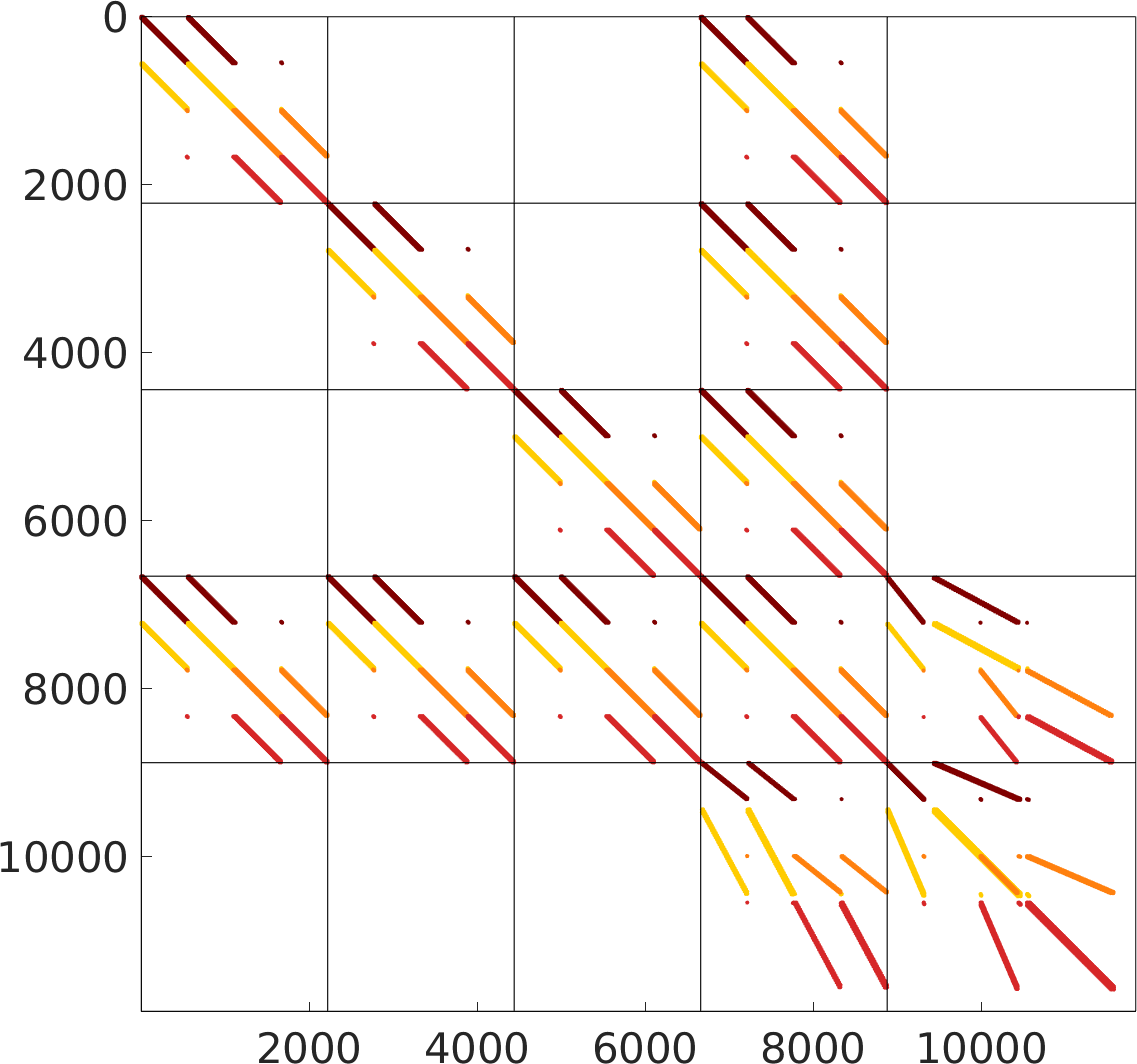
\includegraphics[width=\textwidth]{images/implementation/original_matrix.png}
    \caption{Original matrix layout}%
    \label{fig:original_matrix}%
  \end{subfigure}
  \,
  \begin{subfigure}[t]{0.49\textwidth}%
    \centering%
    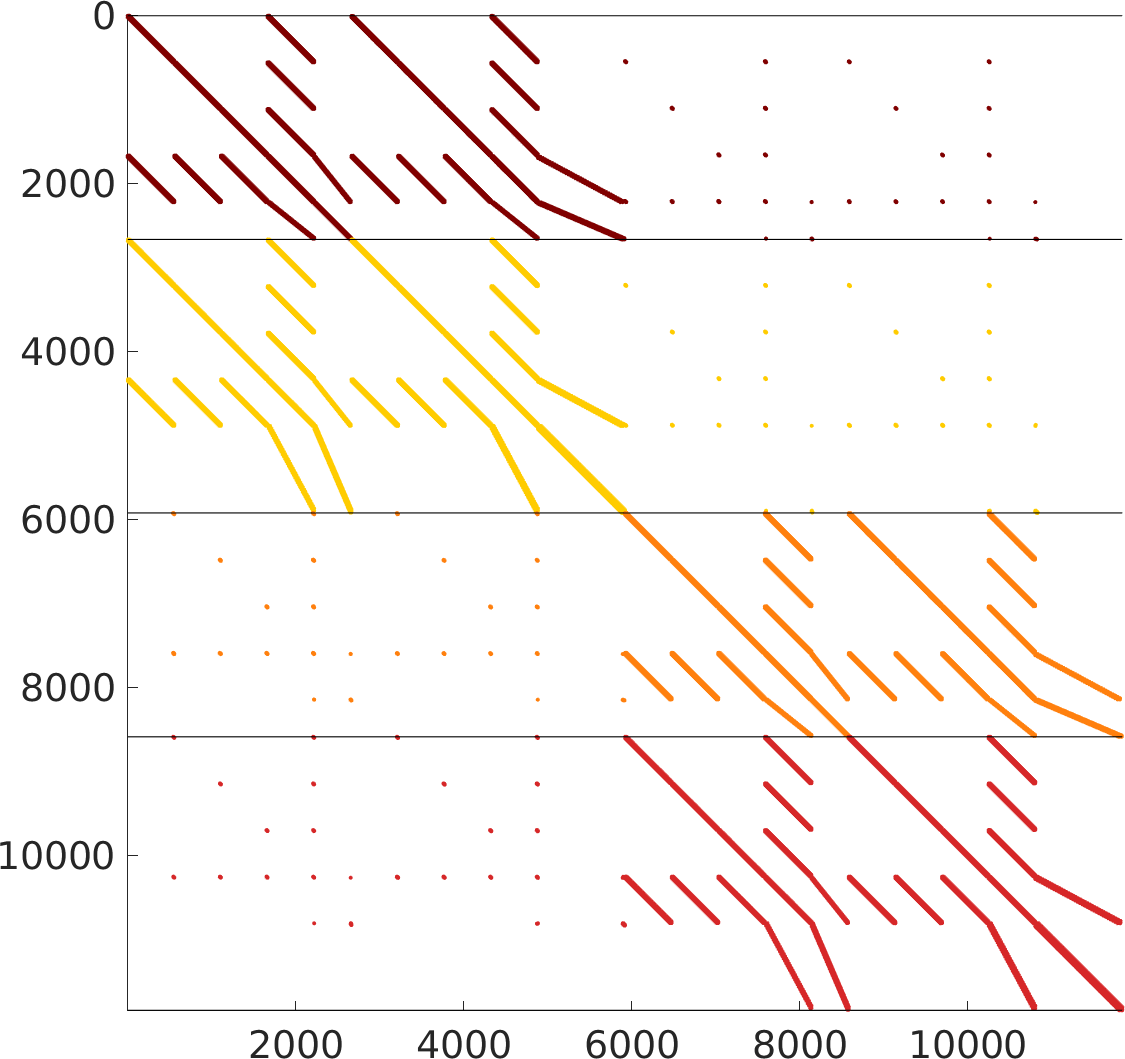
\includegraphics[width=\textwidth]{images/implementation/reordered_matrix.png}
    \caption{Reordered matrix layout}%
    \label{fig:reordered_matrix}%
  \end{subfigure}
  \caption{Nonzero structure of the system matrix of the multidomain problem.}%
  \label{fig:original_reordered_matrix}%
\end{figure}%

\subsection{Properties of a Diagonal Block-Matrix for the Preconditioner}
With the reordered matrix, the linear system can now be solved using almost any preconditioner and linear solver of the PETSc framework. 
For the construction of the preconditioner $\mathcal{P}$ with left preconditioning matrix $P=\mathcal{P}(A)$, we can either use the system matrix $A$ or provide a different matrix $A'$. The preconditioned linear system $P^{-1}A$ should have a smaller condition number than $A$ and, thus, solving the preconditioned system iteratively should be significantly faster than the original $A$ system.

To compute the condition number of the system matrix $A$, we determine its spectrum. \Cref{fig:eigenvalues} shows the real parts of all eigenvalues of $A$. The imaginary parts vanish for almost all eigenvalues. The matrix is singular with one zero-eigenvalue. This property corresponds to the fact that the membrane potential in the problem is abitrary with respect to a constant offset. The singular problem can be solved using appropriate iterative solvers.

% eigenvalues, spectrum, condition number is bad -> preconditioning
The real parts of the eigenvalues are all negative, which is in line with the fact that the model consists of a combination of several diffusion problems. The progression in \cref{fig:eigenvalues} shows a large difference between the largest and the smallest eigenvalues. The condition number of $A$ can be computed by $\textrm{cond}(A) = |\lambda_\text{max}| / |\lambda_\text{min}| = 161.2576 / 0.0116 \approx \num{1.4e5}$. Thus, the problem is ill-conditioned and can benefit from for preconditioning. The condition number is also dependend on the spatial mesh resolution and increases for larger problem sizes.

% PETSc tutorial on preconditioning: https://www.mcs.anl.gov/petsc/meetings/2016/slides/tutorial1.pdf
\begin{figure}
  \centering%
  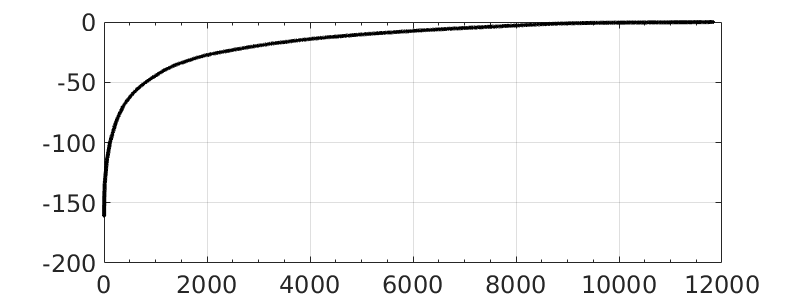
\includegraphics[width=0.6\textwidth]{images/implementation/eigenvalues.png}%
  \caption{Real parts of the eigenvalues sorted by magnitude and corresponding to the example in \cref{fig:multidomain_matrix_mesh}. The non-zero eigenvalue with largest and smallest absolute values are $\lambda_\text{max} = \num{-161.2576}$ and $\lambda_\text{min} = \num{-0.0116}$.}%
  \label{fig:eigenvalues}%
\end{figure}%


% the ten smallest eigenvalues of the matrix:
%     0.0000
%    -0.0116
%    -0.0183
%    -0.0193
%    -0.0204
%    -0.0211
%    -0.0222
%    -0.0229
%    -0.0235
%    -0.0239
% 
% the highest eigenvalues:
%  -161.2576
%  -157.7988
%  -153.7242
%  -151.2197
%  -149.2269
%  -144.5006
%  -143.2441
%  -142.4697
%  -139.5421
%  -139.2625

We experiment with a preconditioning matrix that only uses the diagonal blocks of the system matrix. \Cref{fig:original_diagonal_matrix} shows the non-zero structure of the resulting matrix.
As all diagonal blocks are symmetric matrices, the resulting matrix $A'$ is also symmetric in contrast to $A$. The permutation of rows and columns to obtain the parallel data layout leads to the matrix structure shown in \cref{fig:reordered_diagonal_matrix}. The permutated matrix still contains only diagonal block, because entries in the original diagonal blocks are never permutated out of this block only in their row or column but are always moved by the same permutation in both rows and columns.
\Cref{fig:reordered_diagonal_matrix} shows that the entries on every rank are now decoupled, which potentially allows for a faster computation in the application of the preconditioner.

\begin{figure}%
  \centering%
  \begin{subfigure}[t]{0.49\textwidth}%
    \centering%
    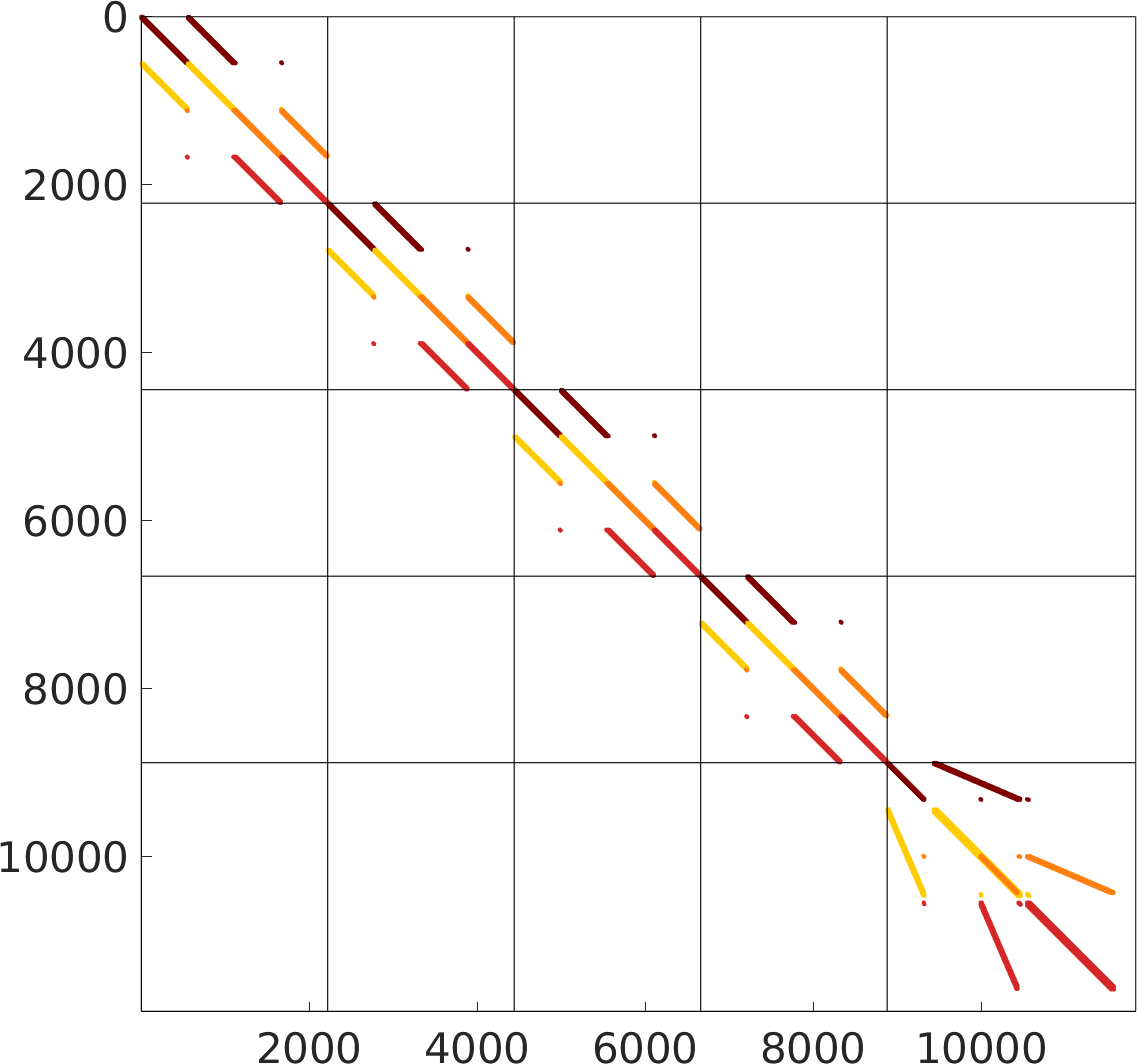
\includegraphics[width=\textwidth]{images/implementation/original_diagonal_matrix.png}
    \caption{Original matrix layout}%
    \label{fig:original_diagonal_matrix}%
  \end{subfigure}
  \,
  \begin{subfigure}[t]{0.49\textwidth}%
    \centering%
    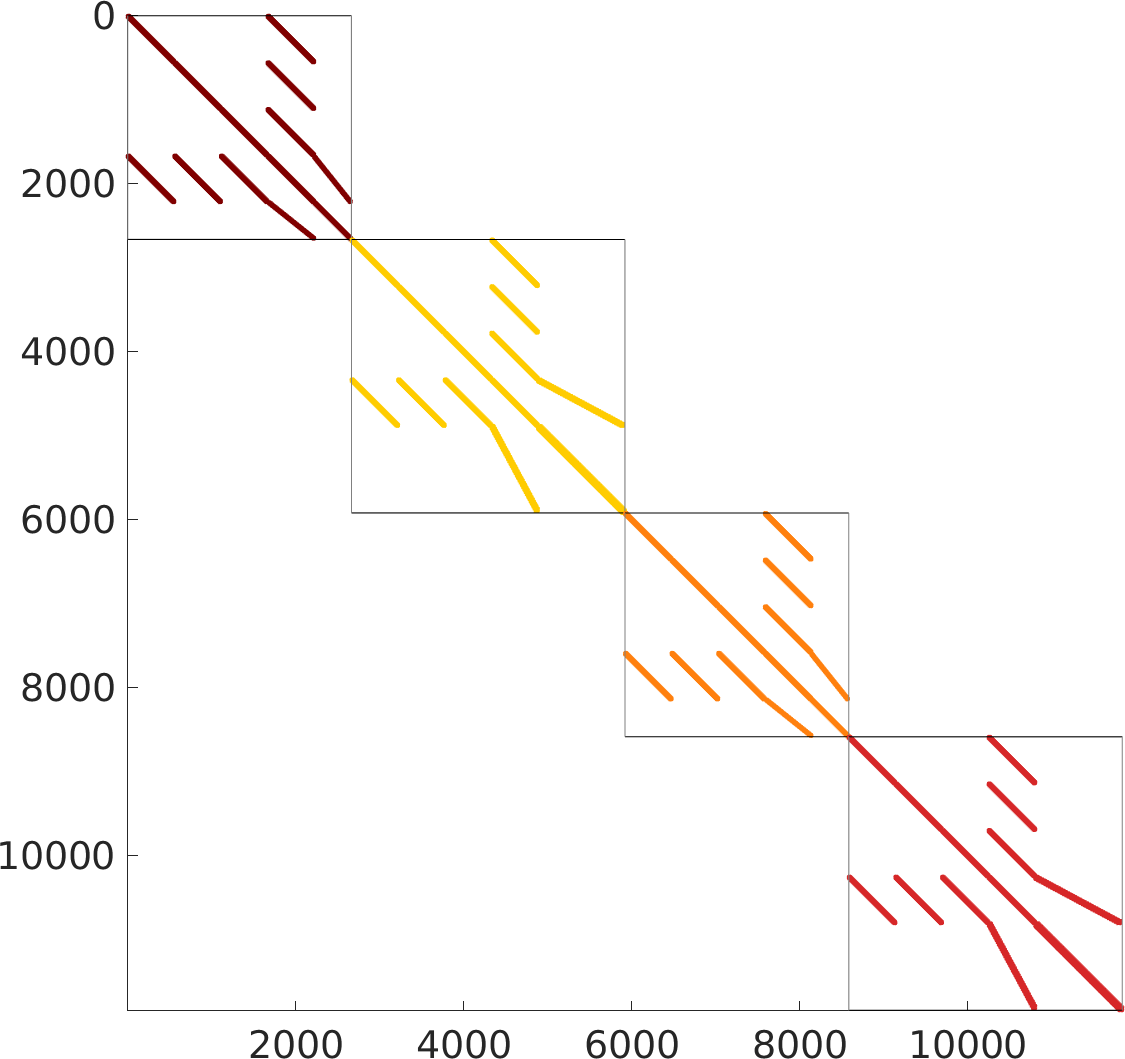
\includegraphics[width=\textwidth]{images/implementation/reordered_diagonal_matrix.png}
    \caption{Reordered matrix layout}%
    \label{fig:reordered_diagonal_matrix}%
  \end{subfigure}
  \caption{Nonzero structure of the symmetric preconditioner matrix of the multidomain problem.}%
  \label{fig:original_reordered_diagonal_matrix}%
\end{figure}%

\subsection{Mesh and Matrices for Higher Degrees of Parallelism}
To show the effect of a higher degree of parallelism on the matrix structure, we also partition the same mesh as in \cref{fig:multidomain_matrix_mesh} to 16 processes. The resulting partitioning of the mesh is given in \cref{fig:16_multidomain_matrix_mesh}.
\Cref{fig:16_original_reordered_diagonal_matrix} shows the non-zero structure of the system matrix and the diagonal matrices for the preconditioner. \Cref{fig:16_original_matrix} contains the original matrix structure that is permutated to the structure in \cref{fig:16_reordered_matrix}. Reordering only the diagonal blocks of the original matrix in \cref{fig:16_original_diagonal_matrix} leads to the structure in \cref{fig:16_reordered_diagonal_matrix}. 
A comparison with \cref{fig:original_reordered_diagonal_matrix} shows that the width of the non-zero band decreases for higher parallelizations.


\begin{figure}
  \centering%
  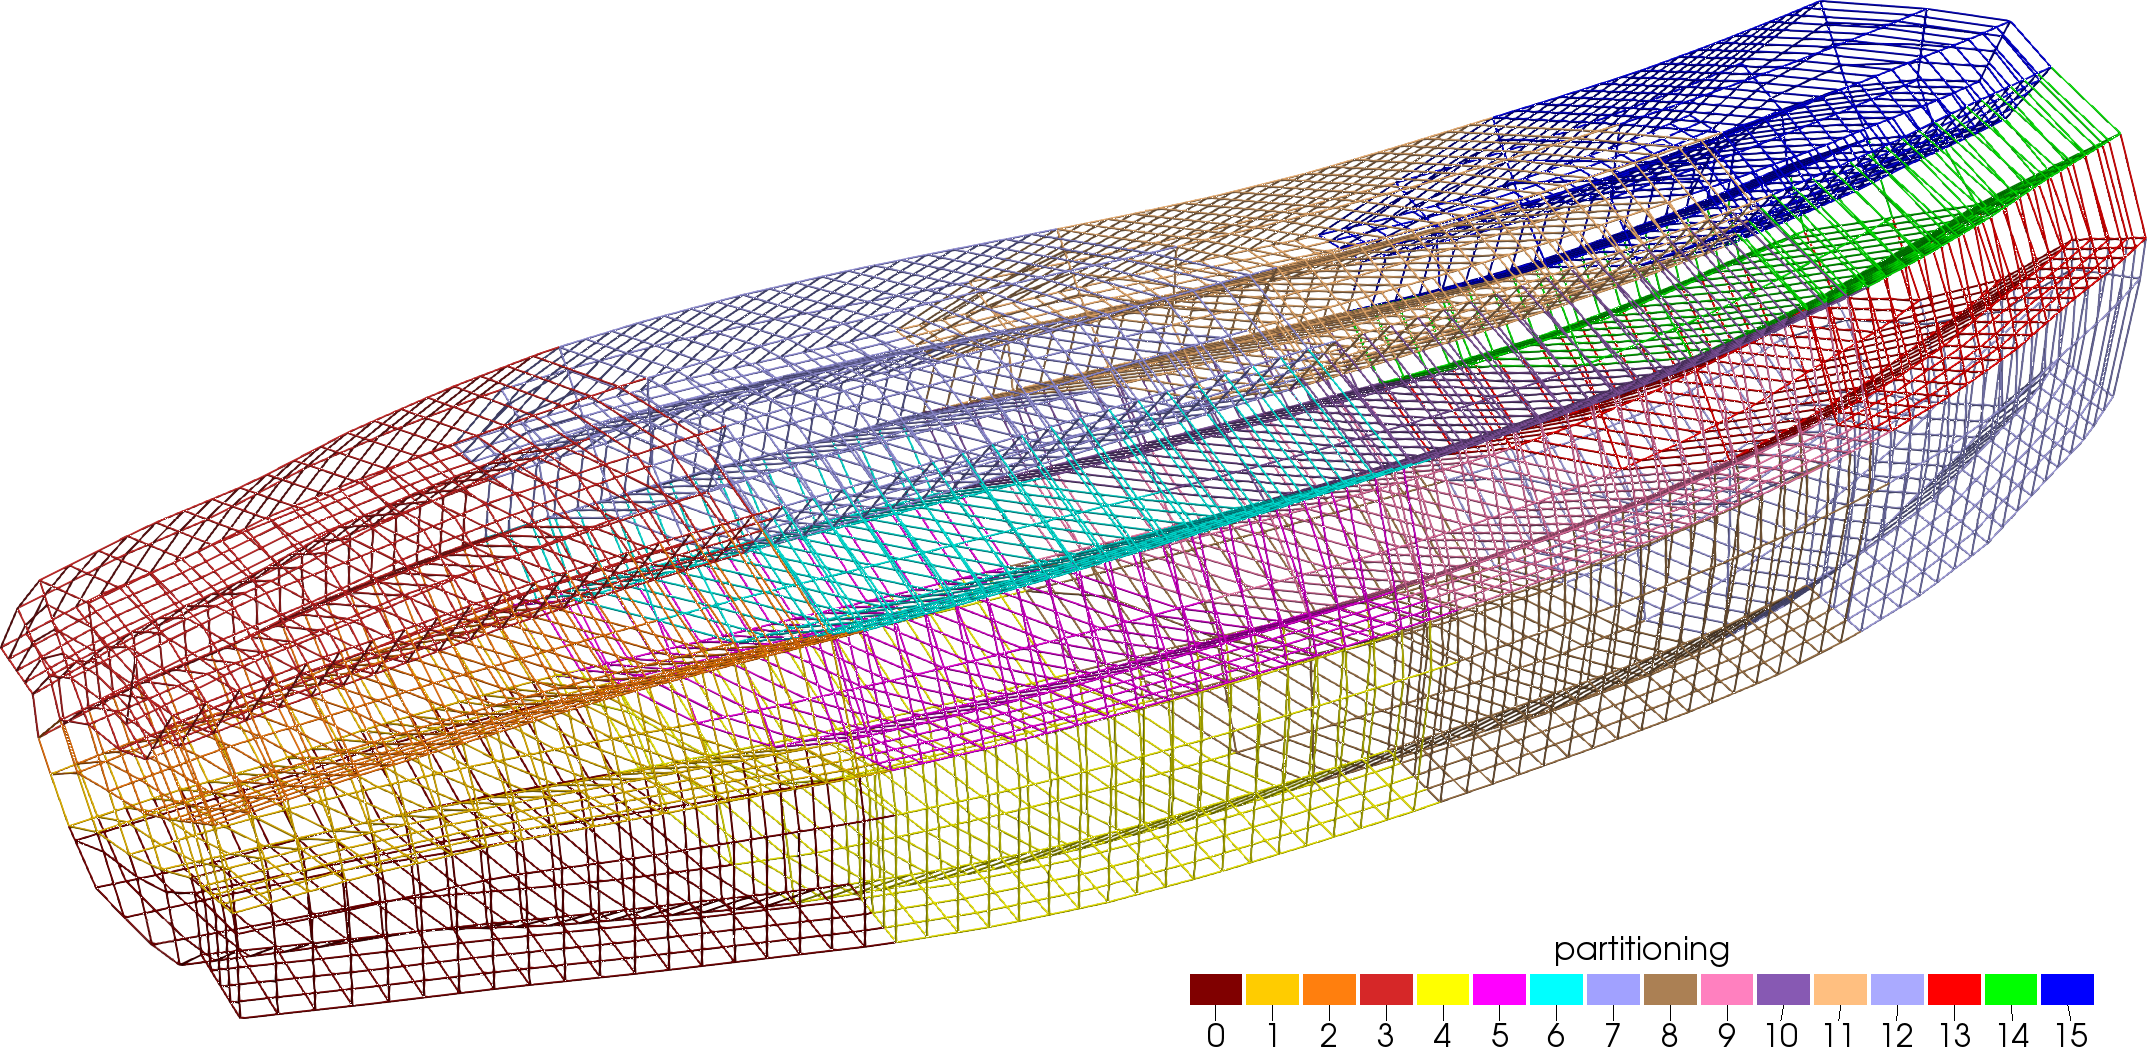
\includegraphics[width=\textwidth]{images/implementation/16_multidomain_matrix_mesh.png}%
  \caption{Partitioning to 16 processes of the mesh in the multidomain example.}%
  \label{fig:16_multidomain_matrix_mesh}%
\end{figure}%

\begin{figure}%
  \centering%
  \begin{subfigure}[t]{0.49\textwidth}%
    \centering%
    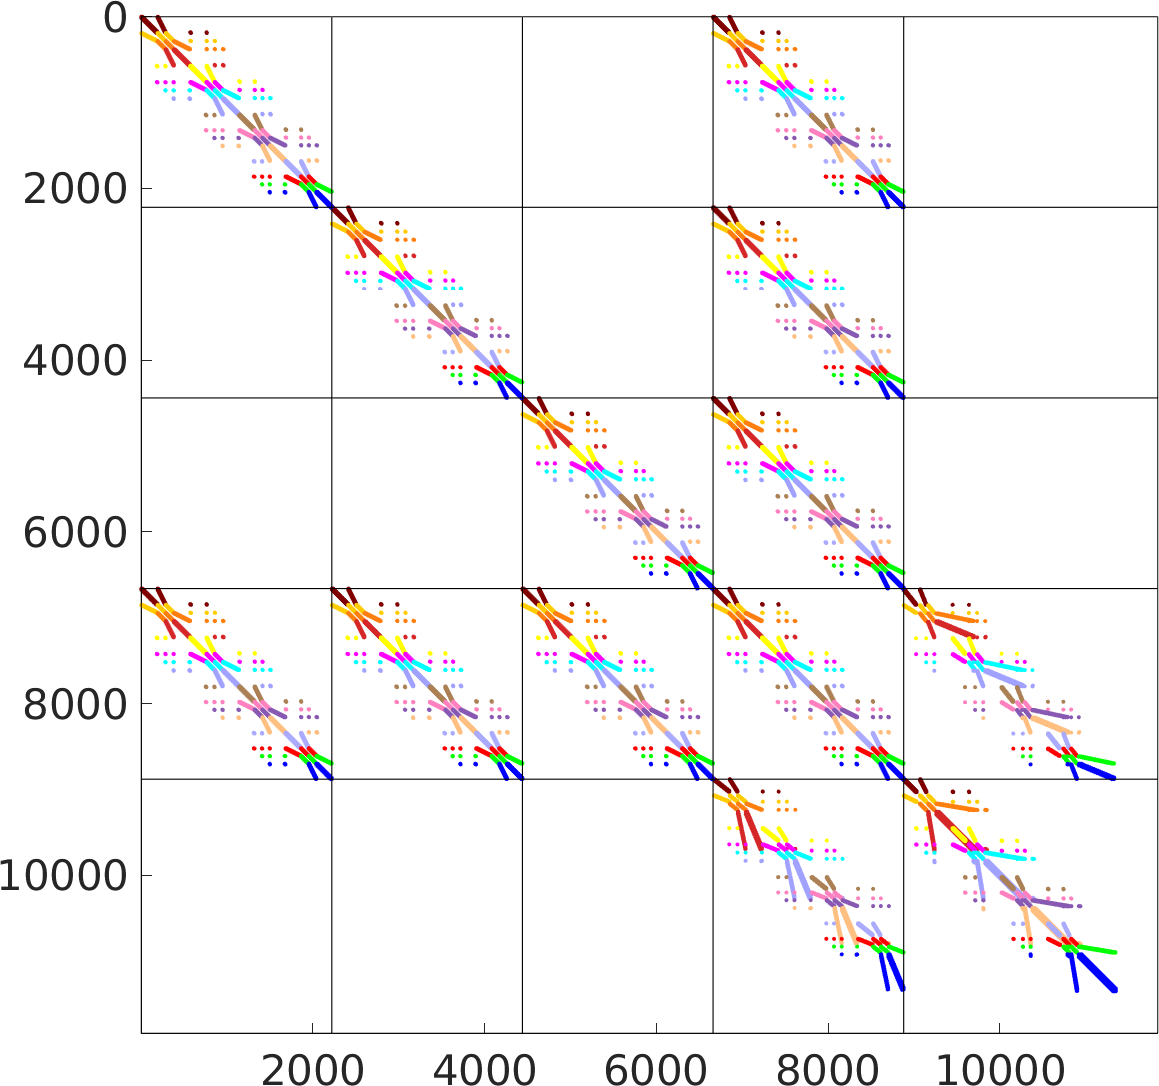
\includegraphics[width=\textwidth]{images/implementation/16_original_matrix.png}
    \caption{Original matrix layout}%
    \label{fig:16_original_matrix}%
  \end{subfigure}
  \,
  \begin{subfigure}[t]{0.49\textwidth}%
    \centering%
    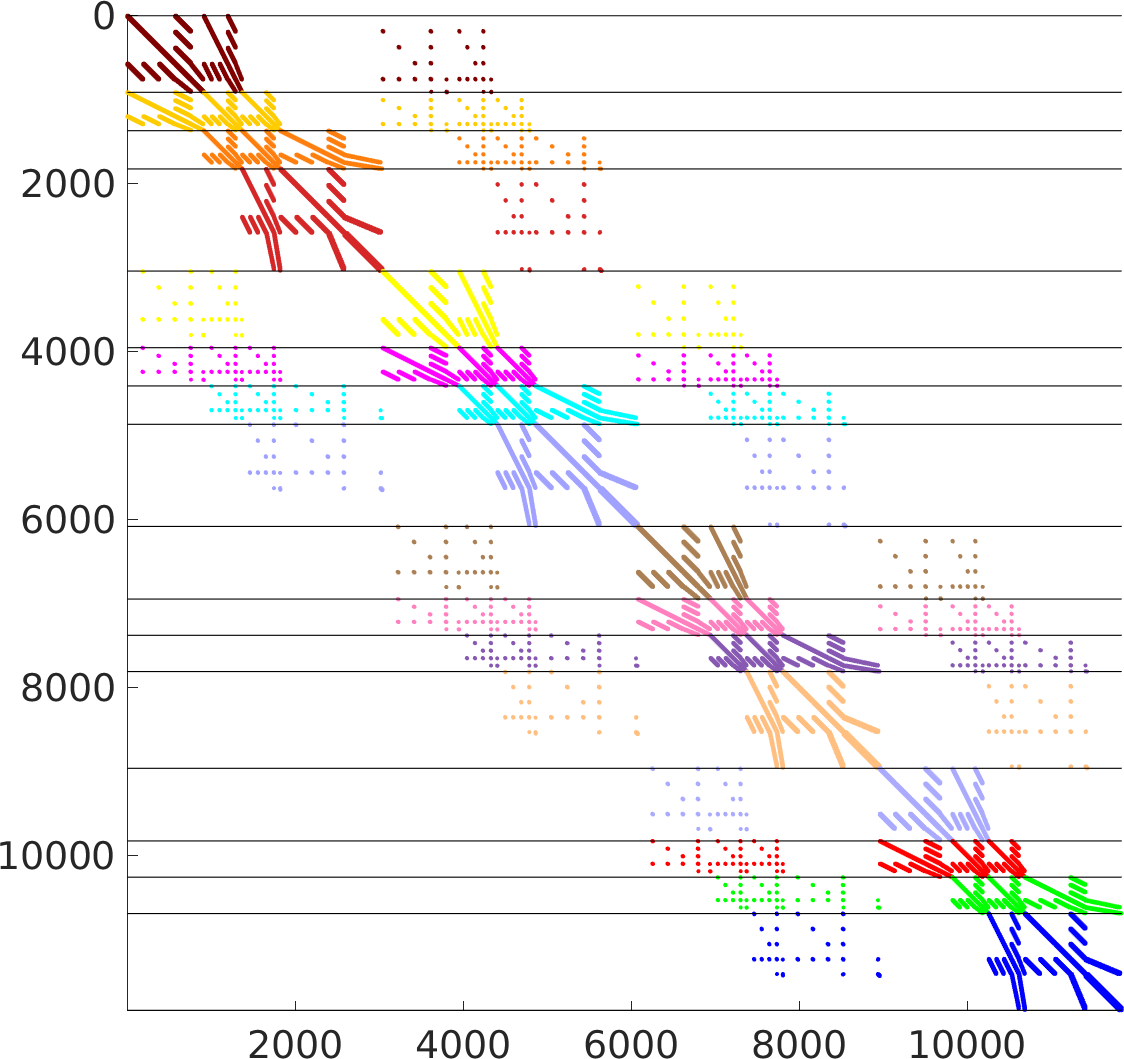
\includegraphics[width=\textwidth]{images/implementation/16_reordered_matrix.png}
    \caption{Reordered matrix layout}%
    \label{fig:16_reordered_matrix}%
  \end{subfigure}
  \\
  \begin{subfigure}[t]{0.49\textwidth}%
    \centering%
    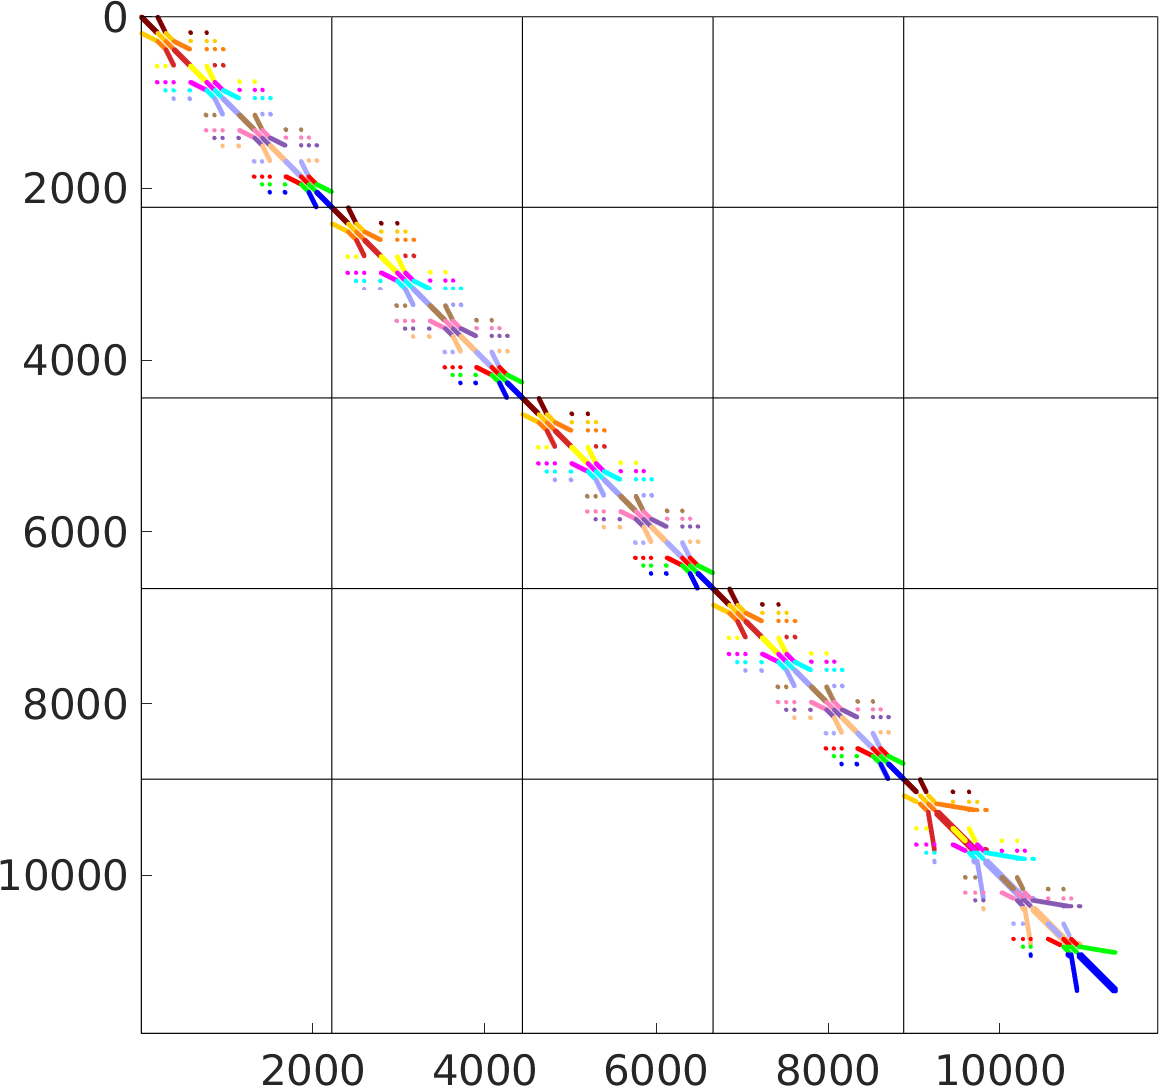
\includegraphics[width=\textwidth]{images/implementation/16_original_diagonal_matrix.png}
    \caption{Original matrix layout}%
    \label{fig:16_original_diagonal_matrix}%
  \end{subfigure}
  \,
  \begin{subfigure}[t]{0.49\textwidth}%
    \centering%
    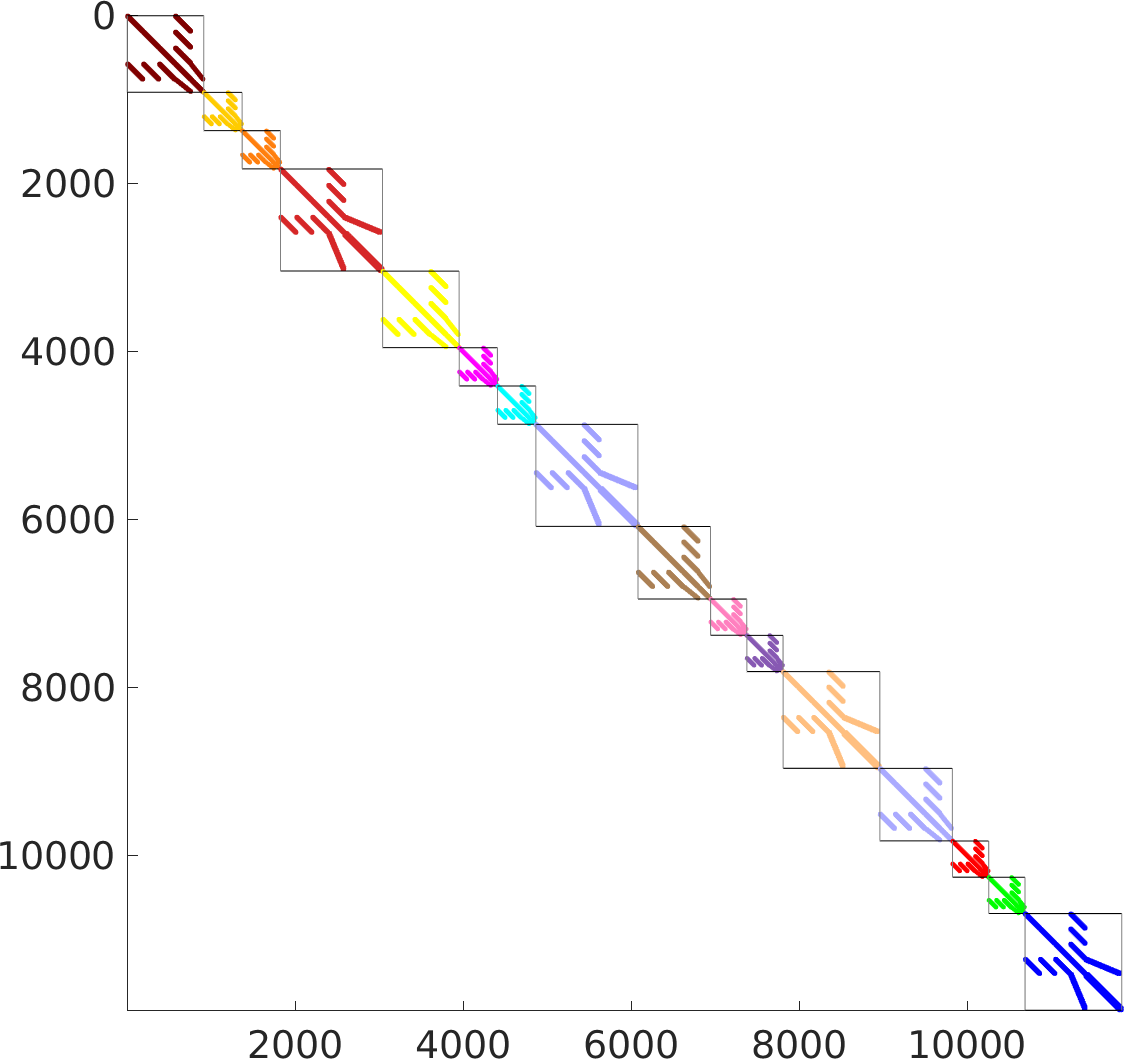
\includegraphics[width=\textwidth]{images/implementation/16_reordered_diagonal_matrix.png}
    \caption{Reordered matrix layout}%
    \label{fig:16_reordered_diagonal_matrix}%
  \end{subfigure}
  \caption{Nonzero structure of the symmetric preconditioner matrix of the multidomain problem partitioned to 16 processes.}%
  \label{fig:16_original_reordered_diagonal_matrix}%
\end{figure}%

\begin{reproduce_no_break}
  The following commands run one timestep of the multidomain simulation with fat layer:
  \begin{lstlisting}[columns=fullflexible,breaklines=true,postbreak=\mbox{\textcolor{gray}{$\hookrightarrow$}\space}]
    cd $\$$OPENDIHU_HOME/examples/electrophysiology/multidomain/multidomain_with_fat/build_release
    mpirun -n 4 ./multidomain_with_fat ../settings_multidomain_with_fat.py matrix.py
    mpirun -n 16 ./multidomain_with_fat ../settings_multidomain_with_fat.py matrix.py
  \end{lstlisting}
  To inspect the system matrix, define a directory where the matrix should be stored. This can be done by setting the parameter \code{config[`Solvers`][`multidomainLinear}\code{Solver`][`dumpFilename`]}, e.g., to \code{`out/matrix/m`}. Then, the directory \code{out/matrix} will contain MATLAB files with the system matrix. To create the plots, open MATLAB, load the system matrix from the  respective file and open the script \code{display_matrix}\code{_entries.m}. Adjust the name of the matrix variable in the first code block, the run the desired steps of the Live Script to produce various plots.\\
  The saved file contains the system matrix already in the reordered layout shown in \cref{fig:reordered_matrix,fig:16_reordered_matrix}. The MATLAB script reverses the permutation that was applied in OpenDiHu to generate the plots of \cref{fig:original_matrix,fig:16_original_matrix}.
\end{reproduce_no_break}

% scenario_name: matrix,  n_subdomains: 4 1 4,  n_ranks: 16,  end_time: 0.002
% dt_0D:           1e-03    multidomain solver:         1000 it. of gmres (10000 it. of gmres), lumped mass matrix: False, initial guess: previous solution
% dt_multidomain:  1e-03    multidomain preconditioner: euclid (euclid), symmetric precond.: True
% dt_splitting:    1e-03    theta: 1.0, solver tolerances, abs: 1e-15, rel: 1e-15
% fiber_file:              ../../../input/left_biceps_brachii_13x13fibers.bin
% fat_mesh_file:           ../../../input/left_biceps_brachii_13x13fibers.bin_fat.bin
% cellml_file:             ../../../input/hodgkin_huxley_1952.c
% firing_times_file:       ../../../input/MU_firing_times_always.txt
% ********************************************************************************
% 16 ranks, partitioning: x4 x y1 x z4
%   sampling 3D mesh with stride 3 x 3 x 20 
%   distribute_nodes_equally: True
%     linear 3D mesh    nodes global: 6 x 5 x 77 = 2310, local: 2 x 5 x 19 = 190
%     linear 3D mesh elements global: 5 x 4 x 76 = 1520, local: 2 x 4 x 19 = 152
%     fat mesh, n points total:    3850 (10 x 5 x 77), (per process: 2 x 5 x 19 = 190)
% 

% details multidomain solver, reordering of matrix entries

% solver structure of contraction
%\begin{figure}
%  \centering%
%  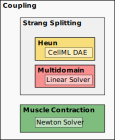
\includegraphics[width=0.5\textwidth]{images/implementation/solver_structure_contraction.pdf}%
%  \caption{solver structure}%
%  \label{fig:prestrech1b}%
%\end{figure}%

% ----

\section{Computation of CellML Models}\label{sec:computation_cellml_models}

In the following, we consider the computation of models that are given in CellML description, such as the subcellular model in the multi-scale muscle model.

The subcellular model is a system of DAEs that is solved at every node of the meshes in the discretized muscle.
For the fiber-based electrophysiology description, instances of the 0D subcellular model are computed on every node of every 1D fiber mesh. The 0D instances are coupled by the monodomain equation on every fiber. For the multidomain description, 0D model instances are solved at every node of the 3D muscle mesh for every compartment.

The subcellular model is provided as a CellML file and can be configured in the Python settings as described in \cref{sec:usage_cellml}.
The \code{CellMLAdapter} is the class in OpenDiHu that computes CellML model instances for all nodes of a given mesh. It computes the expression $G$ of the right hand side of the ODE system to obtain the vector of rates $\partial \bfy / \partial t = G(\bfy)$ and the expression $H$ for the algebraics $\bfh=H(\bfy)$. The new state vector $\bfy$ is computed from the previous vector by using the rates $\partial \bfy / \partial t$ according to a timestepping scheme.  In the solver tree, the timestepping solver class has to be the parent node of the \code{CellMLAdapter}.

CellML models can be obtained as C source files, which can be compiled to shared libraries, loaded and accessed by the solver program. This approach is used is both OpenCMISS and OpenDiHu.
The operation of computing multiple instances of a CellML model at once can be done more efficently than in the naive way of repeatedly executing the model function, as done in OpenCMISS. To exploit the structure of computing multiple model instances together, dedicated C code has to be generated from the CellML model at runtime for given numbers of model instances.
In the following, we describe our code generation functionality for this purpose.

\subsection{Data Flow for the Computation of CellML Models}

\begin{figure}%
  \centering%
  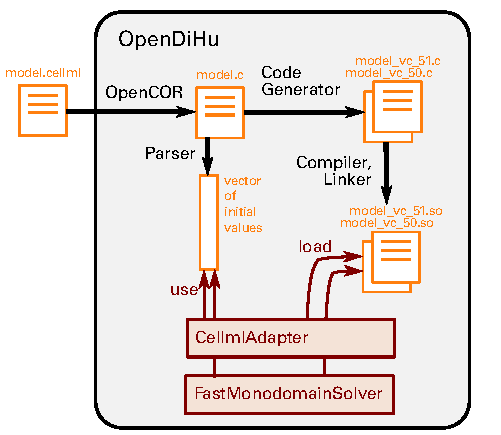
\includegraphics[width=0.7\textwidth]{images/implementation/cellml_scheme.pdf}%
  \caption{Processing of the given CellML model prior to solution. The CellML description is converted to C code using OpenCOR. The parser loads the C source code file and determines the contained initial values. Additionally, it parses the compute instructions into an internal syntax tree. The code generator produces optimizated C code that can solve as many instances of the model as needed on every process according to the global partitioning of the domain. The generated C code is compiled, linked to a shared library and accessed from the solver code.}
  \label{fig:cellml_scheme}%
\end{figure}%

\Cref{fig:cellml_scheme} shows the information flow for the CellML subsystem in OpenDiHu. On the left, a subcellular model is specified in CellML format in a file \code{model.cellml}. OpenDiHu uses the command line interface of OpenCOR to generate corresponding C code in the file \code{model.c}. A parser traverses the file and stores all instructions in an internal syntax tree data structure. The parser also determines the initial values for the state vector $\bfy$ from the code that initializes the variables.
Next, certain constants and algebraics in the compute instructions are replaced by parameter variables, as configured in the settings.

Then, a code generator outputs new C code that is optimized for a given number of CellML instances according to the number of nodes in the processes' subdomain within the global domain decomposition. 
This step is executed in parallel by different processes, but only once for every required number of model instances.

For example, if two fibers with 100 elements each are computed by $2 \times 2$ processes, the 101 nodes on each fiber are equally distributed to two different processes. As a result, each MPI rank has to compute either 51 or 50 CellML instances. Thus, the code generators on two of the ranks produce source code files for 51 and 50 model instances, named \code{model_vc_51.c} and \code{model_vc_50.c} in \cref{fig:cellml_scheme}, respectively. After generation, the source files are each compiled and linked to a shared library, resulting in the shared object files \code{model_vc_51.so} and \code{model_vc_50.so} in \cref{fig:cellml_scheme}.

The generation, compilation and linking steps are performed only by one process per source file.
If a source file or shared library with the required name already exists from a previous run, the steps are omitted.
In the example, only two processes generate and compile the code. All four processes synchronize after all shared libraries have been generated, before proceeding to execute the computations.

The generated shared libraries contain machine-code to compute the functions $G(\bfy)$ and $H(\bfy)$. They are loaded into the simulation program and executed by the \code{CellmlAdapter} class with the corresponding values, as indicated in \cref{fig:cellml_scheme}. Furthermore, the \code{Cellml}\code{Adapter} uses the previously inferred vector of initial values to initialize the state vector before the first timestep. Also the \code{FastMonodomainSolver} class presented in \cref{sec:improved_parallel_solver_for_fiber_based}, which efficiently solves the monodomain equation makes use of the code generator and the shared libraries to execute the subcellular model.

\subsection{Optimizations in the Generated Code}

The code generator can be configured to employ various types of optimizations in the generated code. These optimizations can be selected in the settings by the parameter \code{`optimizationType`}.

The naive way to solve multiple CellML model instances leads to storing the state vectors
in an Array-of-Struct (AoS) memory layout. The \say{struct} containing all components of the state vector for a single CellML model is stored at consecutive locations in memory and multiple structs for all computed instances are lined up next to each other. \Cref{fig:memory_layouts} shows the AoS layout in the top row for four model instances given by different colors. Each instance contains the three state variables $0,1$ and $2$. 

\begin{figure}%
  \centering%
  \begin{subfigure}[t]{0.6\textwidth}%
    \centering%
    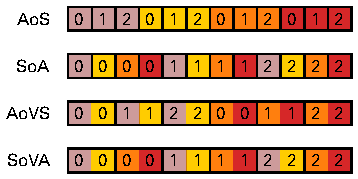
\includegraphics[width=\textwidth]{images/implementation/memory_layouts.pdf}
    \caption{Data in different memory layouts.}%
    \label{fig:memory_layouts}%
  \end{subfigure}\\[4mm]
  \begin{subfigure}[t]{0.7\textwidth}%
    \centering%
    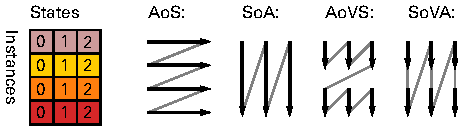
\includegraphics[width=\textwidth]{images/implementation/memory_layouts1.pdf}%
    \caption{Schemes how to construct the memory layouts. On the left, the entries are organized in a 2D field according to the state index and instance index. On the right, the traversal schemes for the different layouts are shown.}%
    \label{fig:memory_layouts1}%
  \end{subfigure}
  \caption{Different memory layouts for the CellML model: Array-of-Struct (AoS), Struct-of-Array (SoA), Array-of-Vectorized-Struct (AoVS), and Struct-of-Vectorized-Array (SoVA). The entries for four instances of the CellML model are shown by different colors and each instance dataset contains the three state variables 0,1 and 2.}%
  \label{fig:memory_layouts_both}%
\end{figure}%

The transposed memory layout is Struct-of-Array (SoA), where the same state components for all model instances are close in memory. In the example in the second row of \cref{fig:memory_layouts}, always four states of the same kind are stored contiguously. 
\Cref{fig:memory_layouts1} shows the construction schemes for the memory layouts. Comparing the scheme for SoA with AoS, it can be seen that the traversal in the 2D field of values is now vertical instead horizontal.

Such a vertical layout is a prerequisite for employing single-instruction-multiple-data (SIMD) parallelism. SIMD instructions perform the same calculations on multiple components of SIMD vectors simultaneously. In the visualization of SoA in \cref{fig:memory_layouts}, always four operands could be loaded simultaneously from memory to the vector registers in the CPU. Modern processors support the AVX2 instruction set with a SIMD lane width of $\mathcal{W}_T=4$ double values or the AVX-512 instruction set with $\mathcal{W}_T=8$ double values.

\begin{figure}
\centering
  \begin{subfigure}[t]{\textwidth}%
  \centering%
\begin{framed}
\begin{lstlisting}[basicstyle=\footnotesize\ttfamily,commentstyle=\color{gray},numbers=left]
  ALGEBRAIC[1] = ( - 0.100000*(STATES[0]+50.0000))/(exp(- (STATES[0]+50.0000)/10.0
  RATES[1] =  ALGEBRAIC[1]*(1.00000 - STATES[1]) -  ALGEBRAIC[5]*STATES[1];
  ...
\end{lstlisting}
\end{framed}
    \caption{Original C code for one CellML model instance generated by OpenCOR.}%
    \label{fig:cellml_codes_original}%
  \end{subfigure}\\[4mm]
  \begin{subfigure}[t]{\textwidth}%
  \centering%
\begin{framed}
\begin{lstlisting}[basicstyle=\footnotesize\ttfamily,commentstyle=\color{gray},numbers=left]
  #pragma omp for simd
  for (int i = 0; i < 1481; i++)
    algebraics[1481+i] = ( - 0.100000*(states[0+i]+50.0000))/(exp(- (states[0+i]+5
    
  #pragma omp for simd
  for (int i = 0; i < 1481; i++)
    rates[1481+i] =  algebraics[1481+i]*(1.00000 - states[1481+i]) -  algebraics[7
  ...
\end{lstlisting}
\end{framed}
    \caption{Generated code for optimization type \code{`simd`}.}%
    \label{fig:cellml_codes_simd}%
  \end{subfigure}\\[4mm]
  \begin{subfigure}[t]{\textwidth}%
  \centering%
\begin{framed}
\begin{lstlisting}[basicstyle=\footnotesize\ttfamily,commentstyle=\color{gray},numbers=left]
  // fill input vectors of states and parameters
  for (int stateNo = 0; stateNo < nStates; stateNo++)
    for (int i = 0; i < nVcVectors; i++)  // Vc vector no
      for (int k = 0; k < $\mathcal{W}_T$; k++)  // entry no in Vc vector 
        statesVc[i*nStates + stateNo][k] = states[stateNo*nInstances + i*$\mathcal{W}_T$+k]; $\label{alg:st_aovs}$
     // statesVc[stateNo*nVcVectors + i][k] = states[stateNo*nInstances + i*$\textcolor{gray}{\mathcal{W}_T}$+k]  $\label{alg:st_sova}$

  for (int i = 0; i < nVcVectors; i++)
  {
    algebraicsVc[i*nAlgebraics + 1] = ( - 0.100000*(statesVc[i*nStates + 0]+50.000 $\label{alg:b_aovs}$
  //algebraicsVc[371+i] = ( - 0.100000*(statesVc[0+i]+50.0000))/(exponential(- (st $\label{alg:b_sova}$
    ...
  }
\end{lstlisting}
\end{framed}
    \caption{Generated code for optimization type \code{`vc`}.}%
    \label{fig:cellml_codes_vc}%
  \end{subfigure}\\[4mm]
  \begin{subfigure}[t]{\textwidth}%
  \centering%
\begin{framed}
\begin{lstlisting}[basicstyle=\footnotesize\ttfamily,commentstyle=\color{gray},numbers=left]
  #pragma omp parallel for
  for (int i = 0; i < 1481; i++)
  {
    algebraics[1481+i] = ( - 0.100000*(states[0+i]+50.0000))/(exp(- (states[0+i]+5
    rates[1481+i] =  algebraics[1481+i]*(1.00000 - states[1481+i]) -  algebraics[7
    ...
  }
\end{lstlisting}
\end{framed}
    \caption{Generated code for optimization type \code{`openmp`}.}%
    \label{fig:cellml_codes_openmp}%
  \end{subfigure}
\caption{Output of the CellML code generator in OpenDiHu for 1481 model instances for different optimization types.  The model is the subcellular model of Hodgkin and Huxley and the code shows only two formulas of this model. Furthermore, the lines are truncated.}%
\label{fig:cellml_codes}%
\end{figure}

\Cref{fig:cellml_codes} demonstrates the code generation and presents different approaches to efficiently compute a CellML model for multiple instances. \Cref{fig:cellml_codes_original} shows the original code for a single model instance, which can be obtained from the CellML website or exported from a CellML model using OpenCOR. The listing shows the computation of the algebraic variable with index one and the rate with index one. The formulas typically use other states, algebraics and constant variables and consist of basic arithmetic such as additions, multiplications, potentiations to integer exponents and exponential functions. Some models, such as the subcellular model of Shorten et al. \cite{shorten2007mathematical} also involve piecewise definitions that include \say{inline if} branching operations.

Calling the code in \cref{fig:cellml_codes_original} for multiple model instances is associated with the AoS memory layout.
An improvement is the generated code with optimization type \code{`simd`} in \cref{fig:cellml_codes_simd}, which assumes the data to be organized in the SoA memory layout. The code is generated specifically to solved 1481 instances of the model. The array indexing for the \code{algebraics} and \code{rates} variables sums the constant offset according to the memory layout and the number of the model instance. For example, for the second algebraic (with former index 1) the offset is 1481 because so many memory locations are filled with values of the first algebraic (with former index 0).

Furthermore, every formula is enclosed in a loop over all 1481 instances of the model. The loops have OpenMP pragmas that instruct the compiler to use SIMD instructions for the loop body, if possible. Because of the consecutive storage, $\mathcal{W}_T$ loop iterations can be combined into a single computation using vector instructions. For the remainder iterations at the end of the loop, the compiler automatically adds different instructions with corresponding smaller SIMD vector lengths.

The approach of using OpenMP pragmas has the advantage that it is independent of the actual hardware capabilities and does not fix the SIMD vector size $\mathcal{W}_T$. If vectorization is disabled at compile-time, sequential CPU code is generated and the same valid solution is computed. A disadvantage is that the performance of the generated code depends on the vectorization ability of the compiler and its detection that the variables have the proper memory layout. For some constructs such as exponential functions or branching instructions, no vectorization is employed and the particular loop falls back to serial code. Such behavior is observed when inspecting the vectorization reports that are emitted by the compiler.

Thus, we implement another optimization type \code{`vc`} in the code generator that guarantees usage of vector instructions for all formulas. We use the C++ library \emph{Vc}, which provides a wrapper to hardware-specific vector instructions and abstracts the SIMD lane width \cite{vc2012,Kretz2015}. Using the data types of this library also allows to write hardware independent code and to achieve performance portability, like with the \code{`simd`} optimization type. 
As \emph{Vc} only supports vectorization up to the AVX2 instruction set, we also use the \code{std::experimental::simd} specification, which is currently considered by the International Organization for Standardization (ISO) and the International Electrotechnical Commission (IEC) for inclusion in the C++ standard library \cite{hoberock2016working}. Switching between these two libraries is transparent in the code and depends on whether the compiler has C++17 support.

Similar to the \code{`simd`} optimization type, the \code{`vc`} optimization type also uses a memory layout where consecutive memory entries correspond to different instances of the model and the traversal direction in \cref{fig:memory_layouts1} is vertical for at least $\mathcal{W}_T$ entries. \Cref{fig:memory_layouts_both} shows two such memory layouts for a SIMD vector length of $\mathcal{W}_T=2$: Array-of-Vectorized-Struct (AoVS) and Struct-of-Vectorized-Array (SoVA). Both are implemented in the code generator. 

The SoVA memory layout is very similar to SoA, the only difference is that in SoVA, entries are always accessed in multiples of the SIMD vector length $\mathcal{W}_T$. The advantage of SoVA is that the array indices are given by the sum of a constant offset with the loop index, whereas with the AoVS layout, a multiplication is required for every access.

AoVS resembles more the AoS layout. Its advantage over SoVA is that the complete state vector $\bfy$ for any model instance is located closer in memory. As the total computation iterates over model instances, the accessed memory is more coherent than for the same iteration scheme with the AoVS layout. This possibly leads to more cache hits, however for set-associative caches, the effect is reduced. Due to the complexity of today's cache architectures, only measurements can decide which of the two memory layouts lead to a faster execution. Our measurements show that the AoVS layout leads to \SI{2}{\percent} shorter runtimes than the SoVA memory layout and, thus, is the preferred choice.

%
%                     subdomains        user  total comp.         0D         1D  bidomain  duration_init     write       mem    n
% scenarioName nRanks                                                                                                            
% vc           18      [3, 2, 3]  186.429444   183.516278  45.524128  95.482744  2.693811       3.053507  1.707781  0.224 GB   18
% vc-aovs      18      [3, 2, 3]  178.800859   177.067879  44.365866  92.375215  2.323516       1.917626  1.673526  0.223 GB  198
% vc-sova      18      [3, 2, 3]  180.776722   179.158511  45.464952  93.226485  2.329576       1.810070  1.685208  0.223 GB  180
% ------------------------------------------------------------------------------------------------------------------------
% 

\Cref{fig:cellml_codes_vc} shows the resulting code using the AoVS memory layout. The commented out lines \ref{alg:st_sova} and \ref{alg:b_sova} show the corresponding code for the SoVA memory layout.
At the beginning of the generated program code, the given data in the \code{states} variable is copied to the \code{statesVc} variable in the new memory layout. Nested loops over all states, over the SIMD vectors and over the scalar values within the SIMD vector are used for this operation. For comparison, lines \ref{alg:st_aovs} and \ref{alg:st_sova} show the corresponding indexing of the \code{statesVc} variables for the AoVS and SoVA memory layouts, respectively.

For the computation of the model, we iterate over the number \code{nVcVectors} of SIMD vectors instead of the number of model instances as for \code{`simd`}. In the example with 1481 instances, we have \code{nVcVectors=$\lceil 1481/\mathcal{W}_T \rceil$=371} SIMD vectors for $\mathcal{W}_T=4$. 
Accordingly, the offsets for indexing the variables in the SoVA layout are smaller, e.g., in line \ref{alg:b_sova} the offset for indexing the \code{algebraicsVc} variables is now 371 instead of 1481 for the non-vectorized variable in the previously considered \code{`simd`} code. 
Comparing the statements for AoVS and SoVA in lines \ref{alg:b_aovs} and \ref{alg:b_sova}, it can be seen that the AoVS memory layout involves an additional multiplication during the indexing of the array.

In case of branching instructions in the CellML formulas, the Vc library provides an implementation of the \say{inline if} statement for SIMD vectors that checks the condition, potentially executes both branches and merges the components from the active branches into the resulting SIMD vector.

Profiling the execution of the \code{`vc`} code for different subcellular models shows that about half of the runtime is spent in evaluating the exponential function. Therefore, we use the following approximation:
\begin{align*}
  \textrm{exp}(x) \approx \textrm{exp}^\ast(x) = \left( 1 + \dfrac{x}{n}\right)^n.
\end{align*}
The series converges to the exact value for $n\to \infty$. We choose $n=1024$ and are able to compute the approximate value by only one addition and 11 multiplications using the following formula:
\begin{align*}
    \textrm{exp}^\ast(x) = \left( 1 + \dfrac{x}{1024}\right)^{2^{10}} = {{{\left( 1 + \dfrac{x}{1024}\right)^2}^2}^{\scriptsize\iddots}}^2.
\end{align*}
%
In the subcellular models of Hodgkin and Huxley \cite{Hodgkin1952} and Shorten et al. \cite{shorten2007mathematical}, the values for $x$ are bounded by $|x| < x_\text{max} = 12$, and we get a relative error of the approximation of $|(\textrm{exp}^\ast - \textrm{exp})(x_\text{max}) / \textrm{exp}(x_\text{max})| < 0.07.$
This approximation can be enabled or disabled in the code generation.

Another optimization is implemented for exponentiation $a^b$. In the considered CellML models, only integer exponents $b\in \mathbb{Z}$ occur. We add a recursive implementation of the power function that requires a logarithmic number of multiplications. 

The code generator with the \code{`vc`} optimization type is also used by the \code{FastMonodomain}\code{Solver} class described in \cref{sec:improved_parallel_solver_for_fiber_based}. The generated codes for the \code{FastMonodomainSolver} class additionally contain the Heun scheme to solve the model, integrate code for the stimulation of muscle fibers and  export certain algebraic values that were declared as parameters in the settings.

Another possiblity to improve the performance besides instruction-level parallelism is thread-level parallelism. The \code{`openmp`} optimization type generates code containing OpenMP pragmas that distribute the computations to multiple OpenMP threads with shared memory. \Cref{fig:cellml_codes_openmp} shows the generated code for this optimization type. A loop iterates over all model instances and the variables are stored in SoA memory layout. The loop iterations are independent of each other as they correspond to different instances of the CellML model. OpenMP distributes the workload to a predefined number of threads that can be specified by environment variables.

\subsection{Code Generation for GPUs}

Besides instruction-level and thread-level parallelism, which were discussed in the last section, accelerator hardware such as GPUs can be considered to reduce the runtime of solving a CellML model.
Our code generator features the \code{`gpu`} optimization type to generate code that is called on the CPU and then offloads the main computations to a GPU.

We use OpenMP 4.5 to instrument the generated code for device offloading. At the time of writing, only an experimental version of GCC 11 is fully capable of compiling this code. In our studies, the code is compiled for the \emph{nvptx} target which generates and compiles device-specific CUDA code using the NVIDIA parallel thread execution (PTX) instruction set architecture. We successfully run the computation on various NVIDIA GPUs, including a GeForce RTX 3080. However, the approach is device-agnostic and other accelerator hardware can also be used.

\Cref{fig:cellml_codes_gpu} shows an excerpt of the generated code. It resembles the code of the\break\code{`openmp`} optimization type, except that the OpenMP pragma in lines \ref{alg:pragma_line} and \ref{alg:pragma_line2} is different. The lines specify the variables to be mapped to and from the target device: The vectors of states and parameters as well as the current simulation time \code{t} are send to the GPU and, after computation, the rates and algebraics are transferred back to the CPU.

\begin{figure}
\centering
\begin{framed}
\begin{lstlisting}[basicstyle=\footnotesize\ttfamily,commentstyle=\color{gray},numbers=left]
  #pragma omp target parallel for \ $\label{alg:pragma_line}$
                     map(to:states,t,parameters) map(from:rates,algebraics) $\label{alg:pragma_line2}$
  for (int i = 0; i < 1481; i++)
  {
    algebraics[1481+i] = ( - 0.100000*(states[0+i]+50.0000))/(exp(- (states[0+i]+5
    rates[1481+i] =  algebraics[1481+i]*(1.00000 - states[1481+i]) -  algebraics[7
    ...
  }
\end{lstlisting}
\end{framed}
\caption{Generated code for optimization type \code{`gpu`} corresponding to the scenario in \cref{fig:cellml_codes}.}%
\label{fig:cellml_codes_gpu}%
\end{figure}

Using the \code{CellmlAdapter}, it is, thus, possible to run any CellML model on the GPU. 
However, for the fiber based electrophysiology model uploading and downloading the data of all model instances between CPU to GPU in every timestep is clearly not the most efficient way to utilize the GPU. Therefore, we add efficient GPU integration with proper memory management to the \code{FastMonodomainSolver} class, which is specialized to solve the monodomain equation for multiple fibers. The class allows to compute multiple timesteps in series on the GPU between subsequent points of synchronization with the CPU. This synchronization is only required, e.g., for writing output files or coupling to a solid mechanics solver.

The generated GPU source code for the \code{FastMonodomainSolver} contains the full algorithm for solving multiple timesteps of the electrophysiology model for multiple fibers with a given number of nodes each. The Strang splitting scheme is used, which solves the 0D subcellular part and the 1D electric conduction part in the scheme 0D-1D-0D.
The 0D part is solved by the Heun scheme. The 1D part is computed either with the implicit Euler method or the Crank-Nicolson method. The linear system of equations is solved using the linear complexity Thomas algorithm.

The parallelization on the GPU uses a fixed number of thread teams, where all threads in a team execute the same code.
For the 0D problem, the iterations of the two nested loops over fibers and model instances per fiber are distributed to all thread teams such that the iterations are \emph{workshared}. Thus, the 0D subcellular models are computed concurrently for all instances. Between the computations of the 0D and 1D parts, synchronization occurs as the data on all instances on a fiber is accessed in the solution of the 1D problem. The 1D computations are distributed on the fiber level, before the second 0D computation in the Strang splitting is again distributed on the model instance level.
Another synchronization occurs after each timestep of the whole Strang splitting.

The data transfer in both directions between CPU and GPU is reduced to a minimum. Initially, all required parameters and initial values have to be transferred to GPU memory. The initial state vector $\bfy$ is only send once to the GPU and all model instances of all fibers get initialized to these same values. Further data to be send includes parameters that describe the stimulation times as presented in \cref{sec:stimulation_times_callbacks}, locations of the neuromuscular junction and the distribution of fibers to motor units. Instead of the callback functions described in \cref{sec:stimulation_times_callbacks}, the stimulation times can be altered by an input file. For details we refer to the online documentation \cite{opendihuWeb}.

During computation, smaller amounts of data are transferred before and after each set of consecutive timesteps on the GPU. The data to be sent to the GPU before the computations consists of the CellML parameter values and the lengths of all elements in the 1D mesh, which change if muscle contraction is computed on the CPU. The data to be transferred back to the CPU after the computations on the GPU consists of a subset of the state vector for every model instance. This subset contains only those components of $\bfy$ that should be written to an output file on the CPU or are required for coupling to another solver. Thus, the majority of the data stays on the GPU.


% ---
\section{Solid Mechanics Solver}\label{sec:solid_mechanics_solver}
Next, we discuss details on the solver of the solid mechanics models, which is needed for the muscle contraction part of the multi-scale model.
\Cref{sec:solver_linear_model_elasticity} gives details on the solver for the linear solid mechanics model. \Cref{sec:specification_of_nonlinear_ma} addresses the nonlinear model and describes how the material model is specified. \Cref{sec:convergence_improvements_for_the_nonlinear_solver} presents the timestepping method for the dynamic problem and describes the implemented measures to improve the convergence.

\subsection{Solver for the Linear Model}\label{sec:solver_linear_model_elasticity}
% linear fem
As noted in \cref{sec:summary_of_existing_solver_classes}, the \code{QuasiStaticLinearElasticitySolver} class can be used to solve the linearized solid mechanics model described in \cref{sec:material_linear_model} and discretized in \cref{sec:linearized_mechanics_model}. 
Within this solver class, the matrix equation \cref{eq:linearized_helper4} is assembled and solved by an object of the \code{FiniteElementMethod} class, which is the same class that is used to solve  Laplace problems.

If the solver is explicitly coupled with an electrophysiology model, we obtain a quasi-static formulation of muscle contraction. The activation parameter $\bar{\gamma}$ on the 3D mesh is transferred from the electrophysiology model to the elasticity model.
Then, the linear system of equations of the elasticity model is solved using the new muscle activation values in the right hand side. The system matrix stays constant in all timesteps. After the new displacements have been computed, the geometries of the 3D mesh and the embedded 1D fiber meshes are updated accordingly.

In this scenario, the active stress tensor $\bfsigma^\text{active}$ in \cref{eq:linearized_helper6} is computed as the product of the activation parameter $\bar{\gamma}$ with a scalar maximum active stress parameter $\sigma_\text{max,active}$ and an anisotropy tensor $\bfa$:
\begin{align}\label{eq:solid_mechanics_solver_1}
  \bfsigma^\text{active} = \sigma_\text{max,active} \,\bar{\gamma}\,\bfa.
\end{align}
The tensor $\bfa$ can be specified in the Python settings by a $3 \times 3$ matrix and allows to specify the anisotropic active behavior of the muscle tissue. In this specification, the first unit vector $\bfe_1=(1,0,0)^\top$ designates the fiber direction, $\bfe_2$ and $\bfe_3$ specify the transverse direction. Prior to the computation in \cref{eq:solid_mechanics_solver_1}, the basis of the given matrix is changed such that $\bfe_1$ in the old basis maps to the fiber direction in the new basis and the new basis is orthonormal. This change of basis is performed at every point in the muscle with the respective fiber direction. Thus, it is possible to specify transversely isotropic material behavior with contraction in fiber direction.

\subsection{Specification of Nonlinear Material Models}\label{sec:specification_of_nonlinear_ma}
% load steps, initalization in the dynamic case

To compute the nonlinear model, the \code{HyperelasticitySolver} class is used for the static formulation of a passive material, the \code{DynamicHyperelasticitySolver} class is used for the dynamic passive behavior and the \code{MuscleContractionSolver} is used for either the static or the dynamic model with active stress contribution.

These solver classes can be coupled to the electrophysiology model in the same way as described in \cref{sec:solver_linear_model_elasticity}.
Similar to \cref{sec:solver_linear_model_elasticity}, the \code{MuscleContractionSolver} adds an active stress term to the formulation according to the formula in \cref{eq:active_stress_term}. The force-length relation $f_\ell(\lambda_f)$ can either be added by the \code{MuscleContractionSolver}  or specified in the CellML description as part of the subcellular model for the activation parameter $\gamma$.

To specify the passive material behavior, the strain energy function $\Psi$ has to be defined.
This definition has to be available at compile-time and is specified in the C++ code. 

Four different terms can be defined to describe the material model in different forms such as the coupled or decoupled representation. The four terms are introduced in \cref{sec:material_modeling} and given in \cref{eq:definition_psi} as follows:
\begin{align}\label{eq:definition_psi1}
  \Psi = \Psi_\text{vol}(J) + \Psi_\text{iso}(\bar{I}_1,\bar{I}_2,\bar{I}_4,\bar{I}_5) + \Psi_1(I_1,I_2,I_3) + \Psi_2(\bfC,\bfa_0).
\end{align}
Formulas for these terms can be specified using C++ expressions with a syntax specified by the \emph{SEMT} library \cite{semt,gutterman2004symbolic} (and also described in the online documentation of OpenDiHu \cite{opendihuWeb}). Mathematical functions such as power and log functions are available, intermediate variables can be defined and reused, and constants for material parameters can be used, whose values can be specified in the Python settings.

The implementation uses the SEMT library to symbolically differentiate the given terms with respect to their function arguments. Thus, all values used in the Newton solver including the Jacobian matrix can be computed automatically. Using this technology, OpenDiHu provides the flexibility to add new material models at compile-time without the need for manual differentiation.

Additionally, three options that alter the computation and efficiency have to be set in the C++ description: The first options specifies whether the material is considered incompressible. If this option is set to true, the solution approach with Lagrange multiplier $p$ is used, otherwise the unknowns only contain the displacements $\bfu$ and possibly the velocities $\bfv$. The second options specifies if the active stress term $\bfS^\text{active}$ should be added to the material. This option is only relevant for the \code{MuscleContractionSolver} class, disabling it allows to compute passive tissue.

The third option determines if the fiber direction $\bfa_0$ appears in the description of the material model. Only if this option is enabled, the corresponding invariants $I_4$ and $I_5$ are available for the definition of the $\Psi_\text{iso}$ term in \cref{eq:definition_psi1}. If disabled, all terms in the formulas in \cref{sec:stress_and_elasticity} that involve $\bfa_0$ are left out of the computation, which speeds up the computations in the solver.

\subsection{Convergence Improvements for the Nonlinear Solver}\label{sec:convergence_improvements_for_the_nonlinear_solver}

The nonlinear equation is solved using the Scalable Nonlinear Equations Solvers (SNES) component of PETSc which provides Newton-type and quasi-Newton methods for solving systems of nonlinear equations. The method to use and other parameters such as the line-search type can be configured in the Python settings file.

Fast convergence of a Newton-based nonlinear solver is facilitated with a good initial guess for the vector of unknowns. Therefore, we predict the solution functions $\bfu$ and $\bfv$ for the next timestep in a dynamic problem using the following computations:
\begin{align*}
  \bfu^{(i+1),\text{predicted}} &= \bfu^{(i)} + \dt\,\bfv^{(i)}, & 
  \bfa^{(i)} &= \dfrac1{\dt}(\bfv^{(i)} - \bfv^{(i-1)}), & 
  \bfv^{(i+1),\text{predicted}} &= \bfv^{(i)} + \dt\,\bfa^{(i)}.
\end{align*}
%
The predicted displacements $\bfu^{(i+1),\text{predicted}}$ for the next timestep $(i+1)$ are estimated by a forward Euler scheme from the displacements $\bfu^{(i)}$ and velocities $\bfv^{(i)}$ of the current timestep $i$. The current acceleration $\bfa^{(i)}$ is estimated by finite differences from the current and previous velocities, $\bfv^{(i)}$ and $\bfv^{(i-1)}$. The predicted velocities $\bfv^{(i+1),\text{predicted}}$ for the next timestep again use a forward Euler method with the estimated acceleration values $\bfa^{(i)}$.
Using the initial guess $(\bfu^{(i+1),\text{predicted}},\bfv^{(i+1),\text{predicted}},p^{(i)})^\top$, the solution vector $(\bfu^{(i+1)},\bfv^{(i+1)},p^{(i+1)})^\top$  for the next timestep can be obtained by the nonlinear system solver.

Independently of the predictions of initial values from previous timesteps, the convergence of the nonlinear solver within a timestep can be  improved by employing load stepping. This approach involves solving $N>1$ sub problems with increasing load steps. In each step $i$, the problem is solved with the right hand side $\bff_i = \alpha_i\,\bff$, scaled by the load factor $\alpha_i \in [0,1]$. The obtained solution in iteration $i$ is used as the initial guess for the subsequent load step $(i+1)$. Increasing values of $\alpha_i$ are used until the final solution is found for $\alpha_N=1$. Typical load factors are $(\alpha_i)_{i=1,\dots,N} = (b^{-(N-1)}, b^{-(N-2)}, \dots, b^{0})$ for a basis $b>0$.

The list of load factors can be specified in the settings. If the nonlinear solver diverges or fails because an unphysical negative determinant $J$ of the deformation gradient occurs, the current load factor is automatically reduced and the solution processes is started again, using the last valid solution as initial guess. If the last successful solution was found for load factor $\alpha_i$ and the current load factor $\alpha_{i+1}$ fails, a new load factor $\alpha^\ast_{i+1} = (\alpha_i + \alpha_{i+1})/2$ is inserted in the list of load factors between $\alpha_i$ and $\alpha_{i+1}$ and the solution of the nonlinear problem with this new factor is attempted. 

In case of a poorly conditioned problem, it can happen that no more solution can be found, regardless of how far the load factor gets decreased. If the difference between two load factors falls below a configurable threshold, the nonlinear solution process for the current timestep is aborted.

Practical tests with the dynamic incompressible problem have shown that the convergence degrades sometimes only for a single timestep and returns to normal in the next timestep. Thus, we allow a single timestep $i$ to diverge and, in this case, continue with the next timestep $(i+1)$ using the (diverged) solution with the lowest residual norm from timestep $i$ to predict the initial guess for timestep $(i+1)$.

